%%%%%%%%%%%%%%%%%%%%%%%%%%%%%%%%%%%%%%%%%%%%%%%%%%%%%%%%%%%%%%%%%%%%%%%%%%%%%%%%%%%%%%%%%%
\begin{document}
\maketitle
%%%%%%%%%%%%%%%%%%%%%%%%%%%%%%%%%%%%%%%%%%%%%%%%%%%%%%%%%%%%%%%%%%%%%%%%%%%%%%%%%%%%%%%%%%

\begin{frame}
 \frametitle{Outline}
  \vspace{-1cm}
  1. Introduction\\[0.1cm]
  2. Mathematical Model\\[0.1cm]
  3. Validation\\[0.1cm]
  4. Results\\[0.1cm]
  5. Conclusion
\end{frame}


%%%%%%%%%%%%%%%%%%%%%%%%%%%%%%%%%%%%%%%%%%%%%%%%%%%%%%%%%%%%%%%%%%%%%%%%%%%%%%%%%%%%%%%%%

\begin{frame}
\frametitle{Introduction}
\vspace{-1.1cm}
\begin{columns}[c]
\column{.6\textwidth}
Motivation:
\begin{itemize}
  \justifying
  \item Ischaemic heart disease and stroke have remained the leading death causes globally in the last 15 years [1]
\end{itemize}
 
\vspace{0.5cm}
 
Aims:
\begin{itemize}
 \justifying
 \item To develop a Finite Element code for stream-vorticity formulation 
       with species transport equation using the Arbitrary Lagrangian-Eulerian (ALE) approach \\


 \vspace{0.2cm}
 \item To create new drug-eluting design patent 

\end{itemize}
\column{.4\textwidth}
\begin{center}
  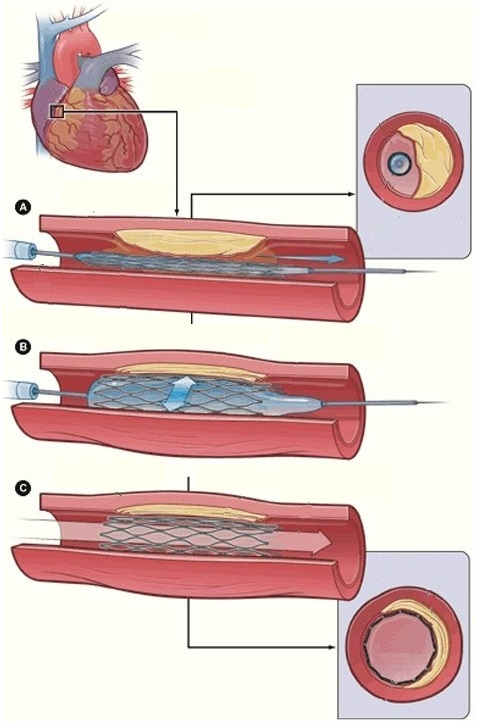
\includegraphics[scale=0.38]{images/stent_bare.jpg}
\end{center}
\end{columns}

\vspace{0.3cm}
\tiny [1] World Health Organization, 2018, "The top 10 causes of death".
\textit{www.who.int/news-room/fact-sheets/detail/the-top-10-causes-of-death}
[Online accessed 06-04-20 08:27pm]



\end{frame}


%%%%%%%%%%%%%%%%%%%%%%%%%%%%%%%%%%%%%%%%%%%%%%%%%%%%%%%%%%%%%%%%%%%%%%%%%%%%%%%%%%%%%%%%%%

\begin{frame}
  \vspace{-1cm}
  \textcolor{gray}{1. Introduction}\\[0.1cm]
  2. Mathematical Model\\[0.1cm]
  \textcolor{gray}{3. Validation}\\[0.1cm]
  \textcolor{gray}{4. Results}\\[0.1cm]
  \textcolor{gray}{5. Conclusion}
\end{frame}

%%%%%%%%%%%%%%%%%%%%%%%%%%%%%%%%%%%%%%%%%%%%%%%%%%%%%%%%%%%%%%%%%%%%%%%%%%%%%%%%%%%%%%%%%%


\begin{frame}
\frametitle{\LARGE Arbitrary Lagrangian-Eulerian (ALE)}

\vspace{-0.4cm}
\begin{columns}[c]
\column{.5\textwidth}
\justifying
The Arbitrary Lagrangian-Eulerian combines
the classical motion descriptions, while it provides [2]:

\vspace{0.5cm}
Advantages:
\begin{itemize}
  \justifying
  \item Simulations in fluid-structure and moving boundary problems
\end{itemize}
 
\vspace{0.5cm}
Disadvantages:
\begin{itemize}
 \justifying
 \item The computational mesh requires an extensive topological treatment
\end{itemize}

\column{.5\textwidth}
\vspace{-1cm}
\begin{center}
\begin{tikzpicture}[scale=0.8]

 % (a) Lagrangian
 % -------------------------------------------------------------------
 % bottom line
 \draw (0,5) -- (6,5);

 \node[square, fill=white, draw, inner sep=0pt, minimum size=8pt] at (0,5) {};
 \node[square, fill=white, draw, inner sep=0pt, minimum size=8pt] at (1,5) {};
 \node[square, fill=white, draw, inner sep=0pt, minimum size=8pt] at (2.7,5) {};
 \node[square, fill=white, draw, inner sep=0pt, minimum size=8pt] at (4,5) {};
 \node[square, fill=white, draw, inner sep=0pt, minimum size=8pt] at (5.1,5) {};
 \node[square, fill=white, draw, inner sep=0pt, minimum size=8pt] at (6,5) {};

 \node[circle, fill=black, inner sep=0pt, minimum size=4pt] at (0,5) {};
 \node[circle, fill=black, inner sep=0pt, minimum size=4pt] at (1,5) {};
 \node[circle, fill=black, inner sep=0pt, minimum size=4pt] at (2.7,5) {};
 \node[circle, fill=black, inner sep=0pt, minimum size=4pt] at (4,5) {};
 \node[circle, fill=black, inner sep=0pt, minimum size=4pt] at (5.1,5) {};
 \node[circle, fill=black, inner sep=0pt, minimum size=4pt] at (6.0,5) {};

 % top line
 \draw (0.5,6) -- (5.4,6);

 \node[square, fill=white, draw, inner sep=0pt, minimum size=8pt] at (0.5,6) {};
 \node[square, fill=white, draw, inner sep=0pt, minimum size=8pt] at (1.4,6) {};
 \node[square, fill=white, draw, inner sep=0pt, minimum size=8pt] at (2.3,6) {};
 \node[square, fill=white, draw, inner sep=0pt, minimum size=8pt] at (3.5,6) {};
 \node[square, fill=white, draw, inner sep=0pt, minimum size=8pt] at (4.6,6) {};
 \node[square, fill=white, draw, inner sep=0pt, minimum size=8pt] at (5.4,6) {};

 \node[circle, fill=black, inner sep=0pt, minimum size=4pt] at (0.5,6) {};
 \node[circle, fill=black, inner sep=0pt, minimum size=4pt] at (1.4,6) {};
 \node[circle, fill=black, inner sep=0pt, minimum size=4pt] at (2.3,6){};
 \node[circle, fill=black, inner sep=0pt, minimum size=4pt] at (3.5,6) {};
 \node[circle, fill=black, inner sep=0pt, minimum size=4pt] at (4.6,6) {};
 \node[circle, fill=black, inner sep=0pt, minimum size=4pt] at (5.4,6) {};

 % mesh motion
 \draw [dashed] (0,  5) -- (0.5,6)  ;
 \draw [dashed] (1,  5) -- (1.4,6)  ;
 \draw [dashed] (2.7,5) -- (2.3,6);
 \draw [dashed] (4,  5) -- (3.5,6)  ;
 \draw [dashed] (5.1,5) -- (4.6,6);
 \draw [dashed] (6,  5) -- (5.4,6)  ;

 % particle motion
 \draw [dotted] (0,  5.15) -- (0.5,5.85);
 \draw [dotted] (1,  5.15) -- (1.4,5.85);
 \draw [dotted] (2.7,5.15) -- (2.3,5.85);
 \draw [dotted] (4,  5.15) -- (3.5,5.85);
 \draw [dotted] (5.1,5.15) -- (4.6,5.85);
 \draw [dotted] (6,  5.15) -- (5.4,5.85):



 % Eulerian legend 
 \draw [latexnew-latex] (-0.3,5) -- (-0.3,6);
 \node at (-0.5,5.5) {t};
 \node at (3,6.5) {\scriptsize Lagrangian description};
 % -------------------------------------------------------------------
 


 % (b) Eulerian
 % -------------------------------------------------------------------
 % bottom line
 \draw (0,2.5) -- (6,2.5);

 \node[square, fill=white, draw, inner sep=0pt, minimum size=8pt] at (0,2.5) {};
 \node[square, fill=white, draw, inner sep=0pt, minimum size=8pt] at (1,2.5) {};
 \node[square, fill=white, draw, inner sep=0pt, minimum size=8pt] at (2.7,2.5) {};
 \node[square, fill=white, draw, inner sep=0pt, minimum size=8pt] at (4,2.5) {};
 \node[square, fill=white, draw, inner sep=0pt, minimum size=8pt] at (5.1,2.5) {};
 \node[square, fill=white, draw, inner sep=0pt, minimum size=8pt] at (6,2.5) {};

 \node[circle, fill=black, inner sep=0pt, minimum size=4pt] at (0,  2.5) {};
 \node[circle, fill=black, inner sep=0pt, minimum size=4pt] at (1,  2.5) {};
 \node[circle, fill=black, inner sep=0pt, minimum size=4pt] at (2.7,2.5) {};
 \node[circle, fill=black, inner sep=0pt, minimum size=4pt] at (4,  2.5) {};
 \node[circle, fill=black, inner sep=0pt, minimum size=4pt] at (5.1,2.5) {};
 \node[circle, fill=black, inner sep=0pt, minimum size=4pt] at (6.0,2.5) {};

 % top line
 \draw (0,3.5) -- (6,3.5);

 \node[square, fill=white, draw, inner sep=0pt, minimum size=8pt] at (0.5,3.5) {};
 \node[square, fill=white, draw, inner sep=0pt, minimum size=8pt] at (1.4,3.5) {};
 \node[square, fill=white, draw, inner sep=0pt, minimum size=8pt] at (2.3,3.5) {};
 \node[square, fill=white, draw, inner sep=0pt, minimum size=8pt] at (3.5,3.5) {};
 \node[square, fill=white, draw, inner sep=0pt, minimum size=8pt] at (4.6,3.5) {};
 \node[square, fill=white, draw, inner sep=0pt, minimum size=8pt] at (5.4,3.5) {};

 \node[circle, fill=black, inner sep=0pt, minimum size=4pt] at (0,  3.5) {};
 \node[circle, fill=black, inner sep=0pt, minimum size=4pt] at (1,  3.5) {};
 \node[circle, fill=black, inner sep=0pt, minimum size=4pt] at (2.7,3.5){};
 \node[circle, fill=black, inner sep=0pt, minimum size=4pt] at (4,  3.5) {};
 \node[circle, fill=black, inner sep=0pt, minimum size=4pt] at (5.1,3.5) {};
 \node[circle, fill=black, inner sep=0pt, minimum size=4pt] at (6.0,3.5) {};

 % mesh motion
 \draw [dashed] (0,  2.5) -- (0,  3.5)  ;
 \draw [dashed] (1,  2.5) -- (1,  3.5)  ;
 \draw [dashed] (2.7,2.5) -- (2.7,3.5)  ;
 \draw [dashed] (4,  2.5) -- (4,  3.5)  ;
 \draw [dashed] (5.1,2.5) -- (5.1,3.5)  ;
 \draw [dashed] (6,  2.5) -- (6,  3.5)  ;

 % particle motion
 \draw [dotted] (0,  2.65) -- (0.5,3.35);
 \draw [dotted] (1,  2.65) -- (1.4,3.35);
 \draw [dotted] (2.7,2.65) -- (2.3,3.35);
 \draw [dotted] (4,  2.65) -- (3.5,3.35);
 \draw [dotted] (5.1,2.65) -- (4.6,3.35);
 \draw [dotted] (6,  2.65) -- (5.4,3.35):



 % Eulerian legend 
 \draw [latexnew-latex] (-0.3,2.5) -- (-0.3,3.5);
 \node at (-0.5,3) {t};
 \node at (3,4.0) {\scriptsize Eulerian description};
 % -------------------------------------------------------------------
 


 % (c) ALE
 % -------------------------------------------------------------------
 % bottom line
 \draw (0,0) -- (6,0);

 \node[square, fill=white, draw, inner sep=0pt, minimum size=8pt] at (0,0) {};
 \node[square, fill=white, draw, inner sep=0pt, minimum size=8pt] at (1,0) {};
 \node[square, fill=white, draw, inner sep=0pt, minimum size=8pt] at (2.7,0) {};
 \node[square, fill=white, draw, inner sep=0pt, minimum size=8pt] at (4,0) {};
 \node[square, fill=white, draw, inner sep=0pt, minimum size=8pt] at (5.1,0) {};
 \node[square, fill=white, draw, inner sep=0pt, minimum size=8pt] at (6,0) {};

 \node[circle, fill=black, inner sep=0pt, minimum size=4pt] at (0,0) {};
 \node[circle, fill=black, inner sep=0pt, minimum size=4pt] at (1,0) {};
 \node[circle, fill=black, inner sep=0pt, minimum size=4pt] at (2.7,0) {};
 \node[circle, fill=black, inner sep=0pt, minimum size=4pt] at (4,0) {};
 \node[circle, fill=black, inner sep=0pt, minimum size=4pt] at (5.1,0) {};
 \node[circle, fill=black, inner sep=0pt, minimum size=4pt] at (6.0,0) {};

 % top line
 \draw (0.2,1) -- (5.8,1);

 \node[square, fill=white, draw, inner sep=0pt, minimum size=8pt] at (0.5,1) {};
 \node[square, fill=white, draw, inner sep=0pt, minimum size=8pt] at (1.4,1) {};
 \node[square, fill=white, draw, inner sep=0pt, minimum size=8pt] at (2.3,1) {};
 \node[square, fill=white, draw, inner sep=0pt, minimum size=8pt] at (3.5,1) {};
 \node[square, fill=white, draw, inner sep=0pt, minimum size=8pt] at (4.6,1) {};
 \node[square, fill=white, draw, inner sep=0pt, minimum size=8pt] at (5.4,1) {};

 \node[circle, fill=black, inner sep=0pt, minimum size=4pt] at (0.2,1) {};
 \node[circle, fill=black, inner sep=0pt, minimum size=4pt] at (1.1,1) {};
 \node[circle, fill=black, inner sep=0pt, minimum size=4pt] at (2.8,1) {};
 \node[circle, fill=black, inner sep=0pt, minimum size=4pt] at (3.8,1) {};
 \node[circle, fill=black, inner sep=0pt, minimum size=4pt] at (4.9,1) {};
 \node[circle, fill=black, inner sep=0pt, minimum size=4pt] at (5.8,1) {};

 % mesh motion
 \draw [dashed] (0,0.0) -- (0.2,1);
 \draw [dashed] (1,0.0) -- (1.1,1);
 \draw [dashed] (2.7,0.0) -- (2.8,1);
 \draw [dashed] (4,0.0) -- (3.8,1);
 \draw [dashed] (5.1,0.0) -- (4.9,1);
 \draw [dashed] (6,0.0) -- (5.8,1);

 % particle motion
 \draw [dotted] (0,0.15) -- (0.5,0.85);
 \draw [dotted] (1,0.15) -- (1.4,0.85);
 \draw [dotted] (2.7,0.15) -- (2.3,0.85);
 \draw [dotted] (4,0.15) -- (3.5,0.85);
 \draw [dotted] (5.1,0.15) -- (4.6,0.85);
 \draw [dotted] (6,0.15) -- (5.4,0.85):



 % ALE legend 
 \draw [latexnew-latex] (-0.3,0) -- (-0.3,1);
 \node at (-0.5,0.5) {t};
 \node at (3,1.5) {\scriptsize ALE description};
 

 % picture legend
 \node[square, draw, inner sep=0pt, minimum size=8pt] at (0.5,-0.7);
 \node[circle, fill=black, inner sep=0pt, minimum size=4pt] at (0.5,-1.2);
 \draw [dotted] (3.5,-0.7) -- (4.08,-0.7);
 \draw [dashed] (3.5,-1.2) -- (4.1,-1.2);

 \node at (1.7,-0.7) {\tiny material point};
 \node at (1.2,-1.2) {\tiny node};
 \node at (5.2,-0.7) {\tiny particle motion};
 \node at (5.1,-1.2) {\tiny mesh motion};
 % -------------------------------------------------------------------


\end{tikzpicture}
\end{center}
\end{columns}

\vspace{0.5cm}
\tiny [2]
Donea, J., Huerta, A., Ponthot, J.‐P. and Rodríguez‐Ferran, A. (2004). Arbitrary Lagrangian–Eulerian Methods. In Encyclopedia of Computational Mechanics \textit{doi:10.1002/0470091355.ecm009}
\end{frame}



%%%%%%%%%%%%%%%%%%%%%%%%%%%%%%%%%%%%%%%%%%%%%%%%%%%%%%%%%%%%%%%%%%%%%%%%%%%%%%%%%%%%%%%%%%

\begin{frame} 
 \frametitle{\LARGE Governing Equations}
\vspace{-1.2cm}
\begin{columns}[c]
\column{.6\textwidth}
Assumptions [3]:\\[0.1cm]
\hspace{0.5cm}  1. Continuum hypothesis\\[0.1cm]
\hspace{0.5cm}  2. Homogeneous and Isotropic\\[0.1cm]
\hspace{0.5cm}  3. Incompressible\\[0.1cm]
\hspace{0.5cm}  4. Newtonian\\[0.1cm]
\hspace{0.5cm}  5. Constant Mass Difusivity\\[0.1cm]
\hspace{0.5cm}  6. Single-phase Flow\\[0.1cm]
\hspace{0.5cm}  7. Two-dimensional flow

\vspace{-1cm}
\column{.4\textwidth}
\begin{center}
\begin{equation*}
 \frac{\partial \omega}{\partial t} + \left( \mathbf{v} - \mathbf{\hat{v}} \right) \cdot \nabla \omega = \frac{1}{Re} \nabla^{2} \omega
\end{equation*}
\medskip
\begin{equation*}
 \nabla^{2} \psi = - \omega
\end{equation*}
\medskip
\begin{equation*}
 \frac{\partial c}{\partial t} + \left( \mathbf{v} - \mathbf{\hat{v}} \right) \cdot \nabla c = \frac{1}{ReSc} \nabla^{2} c 
\end{equation*}
\end{center}
\end{columns}

\vspace{1cm}
\justifying
The material velocity field $\mathbf{v} = \left( v_{x}, v_{y} \right)$ is calculated by: 
$v_{x} = \partial \psi / \partial y$ and 
$v_{y} = - \partial \psi / \partial x$

\bigskip
The mesh velocity field $\mathbf{\hat{v}} \neq \mathbf{v} \left( Lagrangian \right)$ or $0 \left( Eulerian \right)$

\vspace{0.5cm}
\tiny [3]
Batchelor, G. (1967). An Introduction to Fluid Dynamics (Cambridge Mathematical Library). Cambridge: Cambridge University Press. \textit{doi:10.1017/CBO9780511800955}

\end{frame}



%%%%%%%%%%%%%%%%%%%%%%%%%%%%%%%%%%%%%%%%%%%%%%%%%%%%%%%%%%%%%%%%%%%%%%%%%%%%%%%%%%%%%%%%%%
\begin{frame} 
 \frametitle{\LARGE Semi-Lagrangian Method}
\vspace{-1cm}
\begin{columns}[c]
\column{.5\textwidth}
\justifying
The convective term was replaced by material derivative of $\omega$ and $c$ in the direction of characteristic trajectory

\column{.5\textwidth}
\begin{equation*}
 \frac{D \omega}{D t} = \frac{1}{Re} \nabla^{2} \omega
\end{equation*}
\\
\begin{equation*}
 \nabla^{2} \psi = - \omega
\end{equation*}
\\
\begin{equation*}
 \frac{D c}{D t} = \frac{1}{ReSc} \nabla^{2} c 
\end{equation*}
\end{columns}

\vspace{1cm}
\begin{columns}[c]
\column{.5\textwidth}
\justifying
The departure node is calculated by $x_{d}^{n} = x_{i}^{n+1} - \left( \mathbf{v} - \mathbf{\hat{v}}\right) \Delta t$. Then, a searching procedure is required to find $x_{d}^{n}$ using barycentric coordinates



\column{.5\textwidth}
\vspace{-0.5cm}
\begin{center}
\begin{tikzpicture}[scale=2.5]
 % grid
 \draw (2.5,2.5) -- (4.0,2.5);
 \draw (2.5,2.8) -- (4.0,2.8);
 \draw (2.5,3.0) -- (4.0,3.0);

 % material points
 \draw[dashed] (2.8,2.5) -- (3.12,2.8);
 \node[square, fill=white, draw, inner sep=0pt, minimum size=8pt] at (2.8,2.5) {};
 \node[square, fill=white, draw, inner sep=0pt, minimum size=8pt] at (3.12,2.8) {};
 

 % nodes
 \node[circle, fill=black, inner sep=0pt, minimum size=4pt] at (2.60,2.5) {};
 \node[circle, fill=black, inner sep=0pt, minimum size=4pt] at (3.2,2.5) {};
 \node[circle, fill=black, inner sep=0pt, minimum size=4pt] at (3.54,2.5) {};
 \node[circle, fill=black, inner sep=0pt, minimum size=4pt] at (3.85,2.5) {};

 \node[circle, fill=black, inner sep=0pt, minimum size=4pt] at (2.64,2.8) {};
 \node[circle, fill=black, inner sep=0pt, minimum size=4pt] at (3.12,2.8) {};
 \node[circle, fill=black, inner sep=0pt, minimum size=4pt] at (3.64,2.8) {};
 \node[circle, fill=black, inner sep=0pt, minimum size=4pt] at (3.90,2.8) {};

 \node[circle, fill=black, inner sep=0pt, minimum size=4pt] at (2.60,3.0) {};
 \node[circle, fill=black, inner sep=0pt, minimum size=4pt] at (3.1,3.0) {};
 \node[circle, fill=black, inner sep=0pt, minimum size=4pt] at (3.50,3.0) {};
 \node[circle, fill=black, inner sep=0pt, minimum size=4pt] at (3.90,3.0) {};


 % legend
 \node[draw=none, scale=0.8] at (2.80,2.62) {\small $\mathbf{x}_{d}$};
 \node[draw=none, scale=0.8] at (3.22,2.68) {\small $\mathbf{x}_{i}$};

 \node[draw=none, scale=0.8] at (4.10,2.50) {\small $t^{n}$};
 \node[draw=none, scale=0.8] at (4.15,2.80) {\small $t^{n+1}$};
 \node[draw=none, scale=0.8] at (4.15,3.00) {\small $t^{n+2}$};

 \node[draw=none, scale=0.8] at (2.60,2.35) {\small $\mathbf{x}_{i-1}$};
 \node[draw=none, scale=0.8] at (3.12,2.35) {\small $\mathbf{x}_{i}$};
 \node[draw=none, scale=0.8] at (3.64,2.35) {\small $\mathbf{x}_{i+1}$};


\end{tikzpicture}
\end{center}
\end{columns}
\end{frame}





%%%%%%%%%%%%%%%%%%%%%%%%%%%%%%%%%%%%%%%%%%%%%%%%%%%%%%%%%%%%%%%%%%%%%%%%%%%%%%%%%%%%%%%%%%

\begin{frame} 
 \frametitle{\LARGE Semi-Lagrangian Method}

\begin{columns}[c]
\column{.5\textwidth}
\justifying
The implicit semi-Lagrangian time discretization provides [4]:

\medskip
Advantages:
\begin{itemize}
 \justifying
 \item Symmetric linear systems\\
 \item Unconditionnal stability
\end{itemize}

\column{.5\textwidth}
\vspace{-0.5cm}
\begin{equation*}
 \frac{\omega_{i}^{n+1} - \omega_{d}^{n}}{\Delta t} = \frac{1}{Re} \nabla^{2} \omega^{n+1}
\end{equation*}
\begin{equation*}
 \nabla^{2} \psi = - \omega
\end{equation*}
\begin{equation*}
 \frac{c_{i}^{n+1} - c_{d}^{n}}{\Delta t} = \frac{1}{ReSc} \nabla^{2} c^{n+1}
\end{equation*}
\end{columns}

\vspace{0.8cm}
\begin{columns}[c]
\column{.5\textwidth}
\vspace{-0.6cm}
\justifying

Disadvantages:
\begin{itemize}
 \justifying
 \item Numerical Diffusion\\
 \item Searching procedure may lead to excessive computational cost
       if it is not well designed
\end{itemize}


\column{.5\textwidth}
\vspace{-0.5cm}
\begin{center}
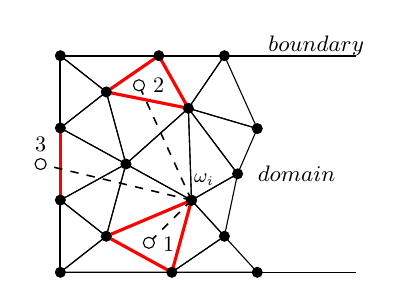
\begin{tikzpicture}[scale=2.5]

 % boundary 
 \draw[line width=0.2mm] (2.5,1.6) -- (4.0,1.6);
 \draw[line width=0.2mm] (2.5,1.6) -- (2.5,0.5);
 \draw[line width=0.2mm] (2.5,0.5) -- (4.0,0.5);

 % nodes
 \coordinate (A) at (2.500,0.5000) {};
 \coordinate (B) at (2.500,0.8667) {};
 \coordinate (C) at (2.500,1.2330) {};
 \coordinate (D) at (2.500,1.6000) {};
 \coordinate (E) at (2.733,0.6830) {};
 \coordinate (F) at (2.833,1.0500) {};
 \coordinate (G) at (2.733,1.4160) {};
 \coordinate (H) at (3.000,1.6000) {};
 \coordinate (I) at (3.066,0.5000) {};
 \coordinate (J) at (3.166,0.8660) {};
 \coordinate (K) at (3.150,1.3330) {};
 \coordinate (L) at (3.333,1.6000) {};
 \coordinate (M) at (3.500,0.5000) {};
 \coordinate (N) at (3.333,0.6830) {};
 \coordinate (O) at (3.400,1.0000) {};
 \coordinate (P) at (3.500,1.2300) {};

 % elements
 \draw (A) -- (E) -- (B) -- cycle;
 \draw (A) -- (I) -- (E) -- cycle;
 \draw (E) -- (J) -- (F) -- cycle;
 \draw (E) -- (F) -- (B) -- cycle;
 \draw (B) -- (F) -- (C) -- cycle;
 \draw (J) -- (K) -- (F) -- cycle;
 \draw (F) -- (K) -- (G) -- cycle;
 \draw (C) -- (F) -- (G) -- cycle;
 \draw (C) -- (G) -- (D) -- cycle;
 \draw (G) -- (H) -- (D) -- cycle;
 \draw (I) -- (N) -- (J) -- cycle;
 \draw (I) -- (M) -- (N) -- cycle;
 \draw (N) -- (O) -- (J) -- cycle;
 \draw (J) -- (O) -- (K) -- cycle;
 \draw (P) -- (L) -- (K) -- cycle;
 \draw (K) -- (L) -- (H) -- cycle;
 \draw (O) -- (P) -- (K) -- cycle;
 \draw[red,line width=0.04cm] (I) -- (J) -- (E) -- cycle;
 \draw[red,line width=0.04cm] (B) -- (C);
 \draw[red,line width=0.04cm] (G) -- (K) -- (H) -- cycle;
 

 % draw nodes
 \node[circle, fill=black, inner sep=0pt, minimum size=4pt] at (A) {};
 \node[circle, fill=black, inner sep=0pt, minimum size=4pt] at (B) {};
 \node[circle, fill=black, inner sep=0pt, minimum size=4pt] at (C) {};
 \node[circle, fill=black, inner sep=0pt, minimum size=4pt] at (D) {};
 \node[circle, fill=black, inner sep=0pt, minimum size=4pt] at (E) {};
 \node[circle, fill=black, inner sep=0pt, minimum size=4pt] at (F) {};
 \node[circle, fill=black, inner sep=0pt, minimum size=4pt] at (G) {};
 \node[circle, fill=black, inner sep=0pt, minimum size=4pt] at (H) {};
 \node[circle, fill=black, inner sep=0pt, minimum size=4pt] at (I) {};
 \node[circle, fill=black, inner sep=0pt, minimum size=4pt] at (J) {};
 \node[circle, fill=black, inner sep=0pt, minimum size=4pt] at (K) {};
 \node[circle, fill=black, inner sep=0pt, minimum size=4pt] at (L) {};
 \node[circle, fill=black, inner sep=0pt, minimum size=4pt] at (M) {};
 \node[circle, fill=black, inner sep=0pt, minimum size=4pt] at (N) {};
 \node[circle, fill=black, inner sep=0pt, minimum size=4pt] at (O) {};
 \node[circle, fill=black, inner sep=0pt, minimum size=4pt] at (P) {};


 % arrow
 \draw[dashed,line width=0.02cm] (J) edge (2.95,0.65);
 \draw[dashed,line width=0.02cm] (J) edge (2.90,1.45);
 \draw[dashed,line width=0.02cm] (J) edge (2.4,1.05) ;

 \node[circle, fill=black, inner sep=0pt, minimum size=4pt] at (J) {};

 % departure nodes
 \node[circle, fill=white, draw, inner sep=0pt, minimum size=4pt] at (2.95,0.65) {};
 \node[circle, fill=white, draw, inner sep=0pt, minimum size=4pt] at (2.90,1.45) {};
 \node[circle, fill=white, draw, inner sep=0pt, minimum size=4pt] at (2.4,1.05) {};


 
 % legend
 \node[draw=none, scale=0.8] at (3.23,0.97) {\small $\omega_{i}$};
 
 \node[draw=none, scale=0.8] at (3.05,0.64) {$1$};
 \node[draw=none, scale=0.8] at (3.00,1.45) {$2$};
 \node[draw=none, scale=0.8] at (2.4,1.15) {$3$};
 
 \node[draw=none, scale=0.9] at (3.7,1.0) {\small $domain$};
 \node[draw=none, scale=0.9] at (3.8,1.65) {\small $boundary$};
\end{tikzpicture}
\end{center}
\end{columns}


\vspace{0.6cm}
\justifying
\tiny [4]
Pironneau, O. On the transport-diffusion algorithm and its applications to the Navier-Stokes equations. Numer. Math. 38, 309–332 (1982). \textit{https://doi.org/10.1007/BF01396435}
\end{frame}



%%%%%%%%%%%%%%%%%%%%%%%%%%%%%%%%%%%%%%%%%%%%%%%%%%%%%%%%%%%%%%%%%%%%%%%%%%%%%%%%%%%%%%%%%%



\begin{frame} 
 \frametitle{\LARGE Galerkin FE Method}
\vspace{-1cm}
\begin{columns}[c]
\column{.5\textwidth}
\begin{figure}[H]
\begin{center}
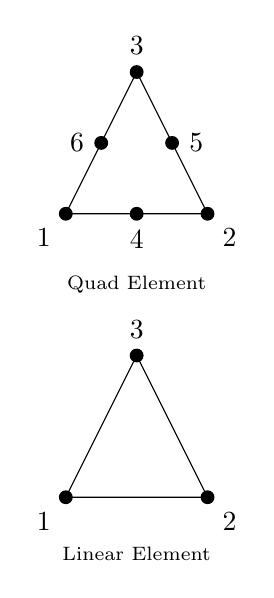
\begin{tikzpicture}[scale=1.8]

 \node at (0.5,1.5) {\scriptsize Quad Element};
 \draw (0,2) -- (1,2) -- (0.5,3) -- cycle;
 \node[circle, fill=black, inner sep=0pt, minimum size=5pt,label=below left:{1}] at (0,2) {};
 \node[circle, fill=black, inner sep=0pt, minimum size=5pt,label=below right:{2}] at (1,2) {};
 \node[circle, fill=black, inner sep=0pt, minimum size=5pt,label=above:{3}] at (0.5,3) {};
 \node[circle, fill=black, inner sep=0pt, minimum size=5pt,label=below:{4}] at (0.5,2) {};
 \node[circle, fill=black, inner sep=0pt, minimum size=5pt,label=right:{5}] at (0.75,2.5) {};
 \node[circle, fill=black, inner sep=0pt, minimum size=5pt,label=left:{6}] at (0.25,2.5) {};

 \node at (0.5,-0.4) {\scriptsize Linear Element};
 \draw (0,0) -- (1,0) -- (0.5,1) -- cycle;
 \node[circle, fill=black, inner sep=0pt, minimum size=5pt,label=below left:{1}] at (0,0) {};
 \node[circle, fill=black, inner sep=0pt, minimum size=5pt,label=below right:{2}] at (1,0) {};
 \node[circle, fill=black, inner sep=0pt, minimum size=5pt,label=above:{3}] at (0.5,1) {};
 


% \draw (-1,0) -- (0,0) -- (-0.5,1) -- cycle;
% \node[circle, fill=black, inner sep=0pt, minimum size=5pt,label=below left:{1}] at (-1,0) {};
% \node[circle, fill=black, inner sep=0pt, minimum size=5pt,label=below right:{2}] at (0,0) {};
% \node[circle, fill=black, inner sep=0pt, minimum size=5pt,label=above:{3}] at (-0.5,1) {};
%
% \draw (1,0) -- (2,0) -- (1.5,1) -- cycle;
% \node[circle, fill=black, inner sep=0pt, minimum size=5pt,label=below left:{1}] at (1,0) {};
% \node[circle, fill=black, inner sep=0pt, minimum size=5pt,label=below right:{2}] at (2,0) {};
% \node[circle, fill=black, inner sep=0pt, minimum size=5pt,label=above:{3}] at (1.5,1) {};
% \node[circle, fill=black, inner sep=0pt, minimum size=5pt,label=above:{4}] at (1.5,0.33) {};



 
 %\node[draw=none, scale=1.2] at (0.5,-0.5) {$N_i = L_i$};
 %\node[draw=none, scale=1.2] at (0.5,-0.9) {$i = 1,2,3$};
\end{tikzpicture}
\end{center}
\end{figure}

\vspace{-1cm}
\column{.5\textwidth}
\begin{center}
\begin{equation*}
 \left[ \frac{\mathbf{M}}{\Delta t} + \frac{\mathbf{K}}{Re} \right] \omega_{i}^{n+1} = \frac{\mathbf{M}}{\Delta t} \omega_{d}^{n}
\end{equation*}
\medskip
\begin{equation*}
 \mathbf{K} \psi = \mathbf{M} \omega
\end{equation*}
\medskip
\begin{equation*}
 \left[ \frac{\mathbf{M}}{\Delta t} + \frac{\mathbf{K}}{ReSc} \right] c_{i}^{n+1} = \frac{\mathbf{M}}{\Delta t} c_{d}^{n}
\end{equation*}
\end{center}
\end{columns}

\vspace{1cm}
\justifying
The material velocity field is calculated by: 
$\mathbf{M} v_{x} = \mathbf{G_{y}} \psi$ and 
$\mathbf{M} v_{y} = - \mathbf{G_{x}} \psi$



\end{frame}

%%%%%%%%%%%%%%%%%%%%%%%%%%%%%%%%%%%%%%%%%%%%%%%%%%%%%%%%%%%%%%%%%%%%%%%%%%%%%%%%%%%%%%%%%%

\begin{frame}
 \frametitle{\LARGE Laplacian Smoothing}

\vspace{-1.2cm}
\begin{columns}[c]
\column{.5\textwidth}
\justifying
To avoid the fast degradation of the computational elements
due to ALE description, it was used the Laplacian Smoothing Method [5]

\bigskip
The new node position $\mathbf{\hat{x}_{i}}$ can be approximated by:

\begin{equation*}
\mathbf{\hat{x}_{i}} = \sum_{i \in N_{1}} e_{ij}^{-1} (\mathbf{x}_{j} - \mathbf{x}_{i})
\end{equation*}

\medskip
where,
$e_{ij}^{-1}$ is the distance between the node and each neighbor in 1-ring $N_{1}$


\vspace{-1cm}
\column{.5\textwidth}
\begin{center}
  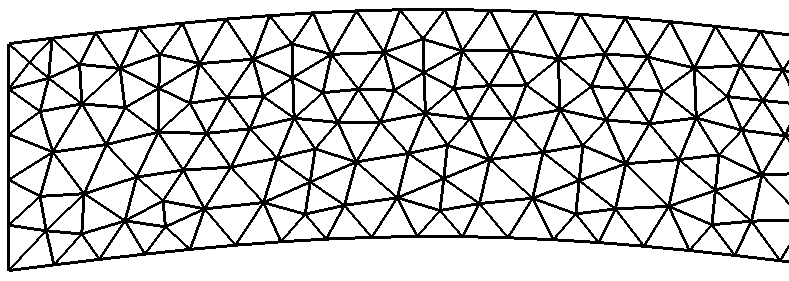
\includegraphics[scale=0.2]{images/Smoothing.png}
  \caption{\scriptsize with Laplacian Smoothing}

  \vspace{1.0cm}
  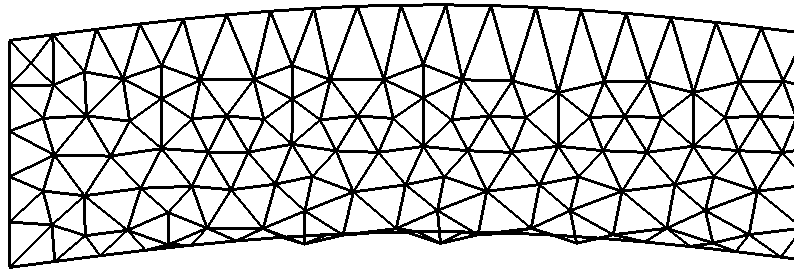
\includegraphics[scale=0.2]{images/noSmoothing.png}
  \caption{\scriptsize no Laplacian Smoothing}
\end{center}
\end{columns}

\vspace{1cm}
\tiny [5] Desbrun,  M.  Meyer,  P.  Schröder,  A.  Barr,  Implicit  fairing  of  irregular  meshes  using  diffusion  and  curvature  flow,  in:  Proceedingsof  Siggraph,  1999,  pp.  317–324

\end{frame}






%%%%%%%%%%%%%%%%%%%%%%%%%%%%%%%%%%%%%%%%%%%%%%%%%%%%%%%%%%%%%%%%%%%%%%%%%%%%%%%%%%%%%%%%%%

\begin{frame} 
 \frametitle{\LARGE Solution Algorithm}
\vspace{-0.5cm}
% Define block styles
\tikzstyle{block} = [rectangle, draw, fill=gray!10!,
    text width=25em, text centered, draw,scale=0.7,text=black!90!]
\tikzstyle{line} = [draw, -latex',scale=0.75]

\begin{center}
\begin{tikzpicture}[node distance = 1.0cm,auto]
    % Place nodes
    \node [block] (step1) {Import mesh};
    \node [block, below of=step1] (step2) {Calculate Gaussian Quadradure and Assemble Matrix};
    \node [block, below of=step2] (step3) {Inicialize Vorticity and Streamfunction};
    \node [block, below of=step3] (step4) {Calculate Laplace smoothing and ALE velocity};
    \node [block, below of=step4] (step5) {Calculate Gaussian Quadradure and Assemble Matrix};
    \node [block, below of=step5] (step6) {Calculate vorticity boundary condition};
    \node [block, below of=step6] (step7) {Calculate semi-Lagrangian and Vorticity field};
    \node [block, below of=step7] (step8) {Calculate streamfunction field};
    \node [block, below of=step8] (step9) {Calculate velocity field};
    \node [block, below of=step9] (step10) {Calculate concentration field};
    \node [right of=step4, node distance=4cm] (initialLoop) {};
    \node [right of=step10, node distance=4cm] (finalLoop) {};
    \node [right of=step7, node distance=5.5cm] (textLoop) {};

    \node [draw=none, align=center,scale=0.7,text=black!80!] at (textLoop) {Repeat the procedure \\ for the next time step \\ until the steady state};
    % Draw edges
    \path [line] (step1) -- (step2);
    \path [line] (step2) -- (step3);
    \path [line] (step3) -- (step4);
    \path [line] (step4) -- (step5);
    \path [line] (step5) -- (step6);
    \path [line] (step6) -- (step7);
    \path [line] (step7) -- (step8);
    \path [line] (step8) -- (step9);
    \path [line] (step9) -- (step10);
    \path [line,dashed] (step10) -- (finalLoop) -- (initialLoop) |- (step4);
\end{tikzpicture}
\end{center}
\end{frame}

%%%%%%%%%%%%%%%%%%%%%%%%%%%%%%%%%%%%%%%%%%%%%%%%%%%%%%%%%%%%%%%%%%%%%%%%%%%%%%%%%%%%%%%%%%

\begin{frame}
  \vspace{-1cm}
  \textcolor{gray}{1. Introduction}\\[0.1cm]
  \textcolor{gray}{2. Mathematical Model}\\[0.1cm]
  3. Validation\\[0.1cm]
  \textcolor{gray}{4. Results}\\[0.1cm]
  \textcolor{gray}{5. Conclusion}
\end{frame}


%%%%%%%%%%%%%%%%%%%%%%%%%%%%%%%%%%%%%%%%%%%%%%%%%%%%%%%%%%%%%%%%%%%%%%%%%%%%%%%%%%%%%%%%%%
\iffalse
\begin{frame}
 \frametitle{\small Validation - Poiseuille Flow}
\vspace{-0.7cm}
\begin{center}
\begin{columns}[c]
\begin{column}{0.55\textwidth} 
\small
Boundaries Conditions:\\[0.2cm]
Inflow condition: $u=1$, $v=0$ e $\psi=y$\\[0.1cm]
Outflow condition: $\psi=y$\\[0.1cm]
Top plate: $u=0$, $v=0$, $\psi=1$\\[0.1cm]
Bottom plate: $u=0$, $v=0$, $\psi=0$
\end{column}
\begin{column}{0.35\textwidth} 
\begin{tikzpicture}[scale=0.8]
 \draw [pattern=north east lines] (0,0) -- (0,-0.1) -- (5,-0.1) -- (5,0) -- cycle;
 \draw [pattern=north east lines] (0,1) -- (0,1.1) -- (5,1.1) -- (5,1) -- cycle;
 \draw [dotted] (0,0.9) -- (5,0.9);
 \draw [dotted] (0,0.7) -- (5,0.7);
 \draw [dotted] (0,0.5) -- (5,0.5);
 \draw [dotted] (0,0.3) -- (5,0.3);
 \draw [dotted] (0,0.1) -- (5,0.1);

% \draw [->,thick] (-2,-0.1)--(-2,1.5) node[left] {$y$};
% \draw [->,thick] (-2.1,0)--(-0.5,0) node[below] {$x$};

 \draw  (4.0,0.0) to [bend right=100] (4.0,1.0);
 \draw  (2.5,0.0) to [bend right=100] (2.5,1.0);
 \draw  (1.0,0.0) to [bend right=100] (1.0,1.0);

 \draw [->,thick] (4.0,0.9) to (4.2,0.9);
 \draw [->,thick] (4.0,0.7) to (4.28,0.7);
 \draw [->,thick] (4.0,0.5) to (4.3,0.5);
 \draw [->,thick] (4.0,0.3) to (4.28,0.3);
 \draw [->,thick] (4.0,0.1) to (4.2,0.1);

 \draw [->,thick] (2.5,0.9) to (2.7,0.9);
 \draw [->,thick] (2.5,0.7) to (2.78,0.7);
 \draw [->,thick] (2.5,0.5) to (2.8,0.5);
 \draw [->,thick] (2.5,0.3) to (2.78,0.3);
 \draw [->,thick] (2.5,0.1) to (2.7,0.1);

 \draw [->,thick] (1.0,0.9) to (1.2,0.9);
 \draw [->,thick] (1.0,0.7) to (1.28,0.7);
 \draw [->,thick] (1.0,0.5) to (1.3,0.5);
 \draw [->,thick] (1.0,0.3) to (1.28,0.3);
 \draw [->,thick] (1.0,0.1) to (1.2,0.1);
\end{tikzpicture}
\end{column}
\end{columns}
\end{center}
\vspace{-0.5cm}
\begin{center}
\begin{columns}[c]
\begin{column}{0.4\textwidth} 
\begin{equation*}
u = \frac{4 u_{max}}{L^2} y \big[ L - y \big]
\end{equation*}
\end{column}
\begin{column}{0.73\textwidth} 
\begin{figure}
  \centering
  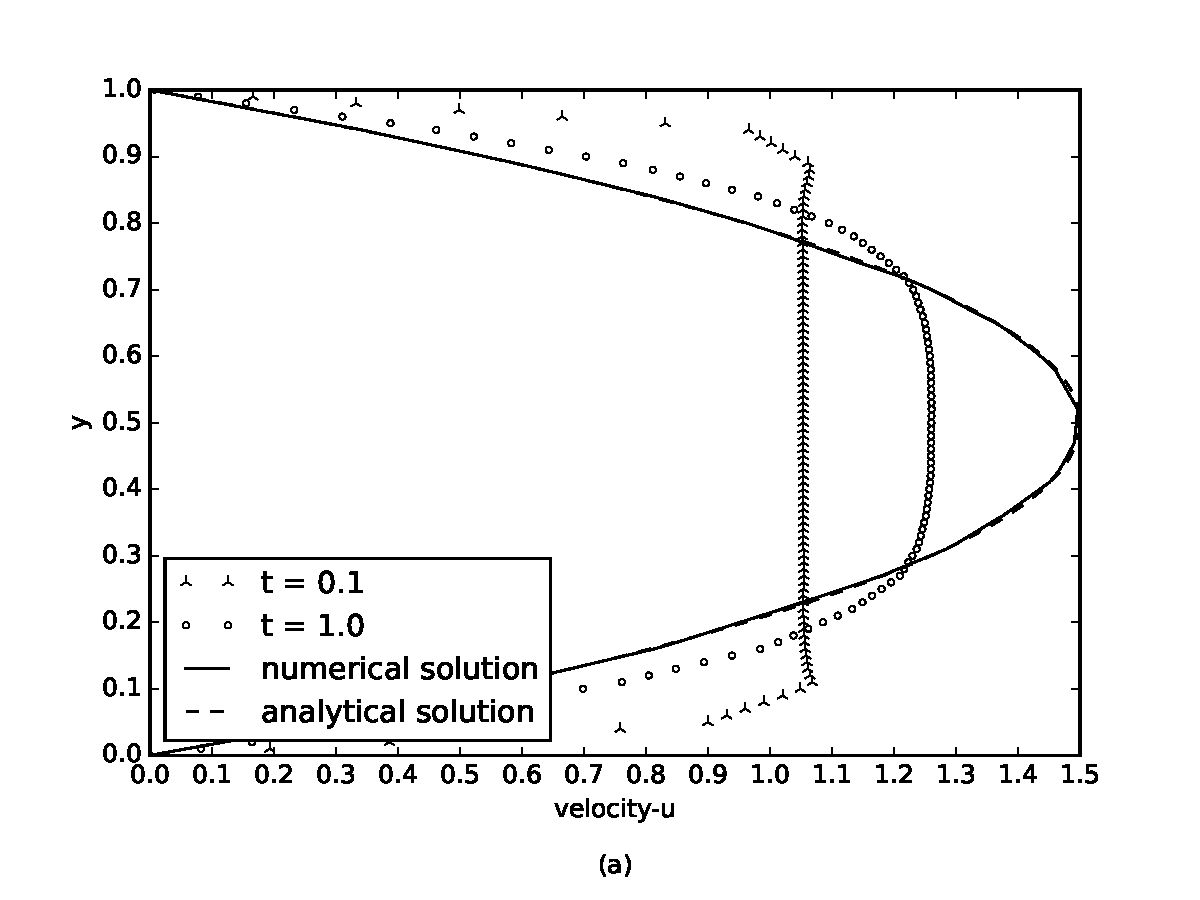
\includegraphics[scale=0.48]{images/poiseuille_velocity.pdf}
\end{figure}
%\vspace{-0.2cm}
%\centering \scriptsize Evolution of velocity field profile in time for \textit{$Re = 100$} and the comparison between numerical solution and analytical solution
\end{column}
\end{columns}
\end{center}
\end{frame}
\fi


%%%%%%%%%%%%%%%%%%%%%%%%%%%%%%%%%%%%%%%%%%%%%%%%%%%%%%%%%%%%%%%%%%%%%%%%%%%%%%%%%%%%%%%%%%

\begin{frame}
 \frametitle{\LARGE Validation - Poiseuille Flow}
\vspace{-0.55cm}
\begin{center}
\begin{columns}[c]
\begin{column}{0.55\textwidth} 
\small
Boundaries Conditions:\\[0.2cm]
Inflow condition: $u=u_{analytical}$, $v=0$
Top plate: $u=0$, $v=0$, $\psi=1$\\[0.1cm]
Bottom plate: $u=0$, $v=0$, $\psi=0$
\end{column}
\begin{column}{0.35\textwidth} 
\begin{tikzpicture}[scale=0.8]
 \draw [pattern=north east lines] (0,0) -- (0,-0.1) -- (5,-0.1) -- (5,0) -- cycle;
 \draw [pattern=north east lines] (0,1) -- (0,1.1) -- (5,1.1) -- (5,1) -- cycle;
 \draw [dotted] (0,0.9) -- (5,0.9);
 \draw [dotted] (0,0.7) -- (5,0.7);
 \draw [dotted] (0,0.5) -- (5,0.5);
 \draw [dotted] (0,0.3) -- (5,0.3);
 \draw [dotted] (0,0.1) -- (5,0.1);

% \draw [->,thick] (-2,-0.1)--(-2,1.5) node[left] {$y$};
% \draw [->,thick] (-2.1,0)--(-0.5,0) node[below] {$x$};

 \draw  (4.0,0.0) to [bend right=100] (4.0,1.0);
 \draw  (2.5,0.0) to [bend right=100] (2.5,1.0);
 \draw  (1.0,0.0) to [bend right=100] (1.0,1.0);

 \draw [->,thick] (4.0,0.9) to (4.2,0.9);
 \draw [->,thick] (4.0,0.7) to (4.28,0.7);
 \draw [->,thick] (4.0,0.5) to (4.3,0.5);
 \draw [->,thick] (4.0,0.3) to (4.28,0.3);
 \draw [->,thick] (4.0,0.1) to (4.2,0.1);

 \draw [->,thick] (2.5,0.9) to (2.7,0.9);
 \draw [->,thick] (2.5,0.7) to (2.78,0.7);
 \draw [->,thick] (2.5,0.5) to (2.8,0.5);
 \draw [->,thick] (2.5,0.3) to (2.78,0.3);
 \draw [->,thick] (2.5,0.1) to (2.7,0.1);

 \draw [->,thick] (1.0,0.9) to (1.2,0.9);
 \draw [->,thick] (1.0,0.7) to (1.28,0.7);
 \draw [->,thick] (1.0,0.5) to (1.3,0.5);
 \draw [->,thick] (1.0,0.3) to (1.28,0.3);
 \draw [->,thick] (1.0,0.1) to (1.2,0.1);
\end{tikzpicture}\\[0.2cm]
\small Nodes: 1757\\
\small Elements: 3263\\
\small Relative Error: 0.67\%
\end{column}
\end{columns}
\end{center}

\vspace{0.2cm}
\begin{center}
\begin{columns}[c]
\begin{column}{0.55\textwidth} 
% This file was created by tikzplotlib v0.9.1.
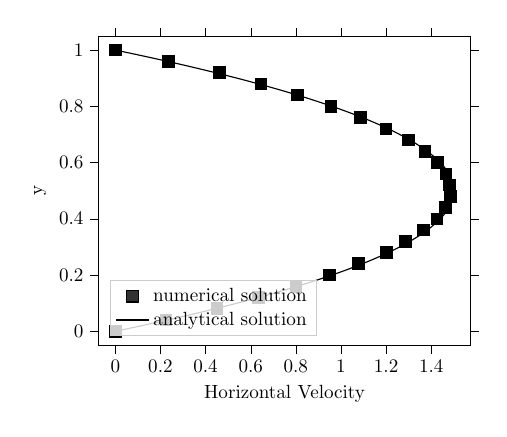
\begin{tikzpicture}[scale=0.69]

\begin{axis}[
legend cell align={left},
legend style={fill opacity=0.8, draw opacity=1, text opacity=1, at={(0.03,0.03)}, anchor=south west, draw=white!80!black},
tick align=outside,
tick pos=both,
x grid style={white!69.0196078431373!black},
xlabel={Horizontal Velocity},
xmin=-0.075, xmax=1.575,
xtick style={color=black},
y grid style={white!69.0196078431373!black},
ylabel={y},
ymin=-0.05, ymax=1.05,
ytick style={color=black}
]
\addplot [semithick, black, mark=square*, mark size=3, mark options={solid}, only marks]
table {%
0 0
0.22464 0.04
0.45077 0.08
0.63337 0.12
0.80061 0.16
0.94904 0.2
1.0779 0.24
1.2022 0.28
1.2864 0.32
1.3668 0.36
1.4249 0.4
1.4633 0.44
1.4849 0.48
1.4797 0.52
1.466 0.56
1.4268 0.6
1.3732 0.64
1.2996 0.68
1.1988 0.72
1.0859 0.76
0.95592 0.8
0.80633 0.84
0.64626 0.88
0.4616 0.92
0.23661 0.96
0 1
};
\addlegendentry{numerical solution}
\addplot [semithick, black]
table {%
0 0
0.02985 0.005
0.0594 0.01
0.08865 0.015
0.1176 0.02
0.14625 0.025
0.1746 0.03
0.20265 0.035
0.2304 0.04
0.25785 0.045
0.285 0.05
0.31185 0.055
0.3384 0.06
0.36465 0.065
0.3906 0.07
0.41625 0.075
0.4416 0.08
0.46665 0.085
0.4914 0.09
0.51585 0.095
0.54 0.1
0.56385 0.105
0.5874 0.11
0.61065 0.115
0.6336 0.12
0.65625 0.125
0.6786 0.13
0.70065 0.135
0.7224 0.14
0.74385 0.145
0.765 0.15
0.78585 0.155
0.8064 0.16
0.82665 0.165
0.8466 0.17
0.86625 0.175
0.8856 0.18
0.90465 0.185
0.9234 0.19
0.94185 0.195
0.96 0.2
0.97785 0.205
0.9954 0.21
1.01265 0.215
1.0296 0.22
1.04625 0.225
1.0626 0.23
1.07865 0.235
1.0944 0.24
1.10985 0.245
1.125 0.25
1.13985 0.255
1.1544 0.26
1.16865 0.265
1.1826 0.27
1.19625 0.275
1.2096 0.28
1.22265 0.285
1.2354 0.29
1.24785 0.295
1.26 0.3
1.27185 0.305
1.2834 0.31
1.29465 0.315
1.3056 0.32
1.31625 0.325
1.3266 0.33
1.33665 0.335
1.3464 0.34
1.35585 0.345
1.365 0.35
1.37385 0.355
1.3824 0.36
1.39065 0.365
1.3986 0.37
1.40625 0.375
1.4136 0.38
1.42065 0.385
1.4274 0.39
1.43385 0.395
1.44 0.4
1.44585 0.405
1.4514 0.41
1.45665 0.415
1.4616 0.42
1.46625 0.425
1.4706 0.43
1.47465 0.435
1.4784 0.44
1.48185 0.445
1.485 0.45
1.48785 0.455
1.4904 0.46
1.49265 0.465
1.4946 0.47
1.49625 0.475
1.4976 0.48
1.49865 0.485
1.4994 0.49
1.49985 0.495
1.5 0.5
1.49985 0.505
1.4994 0.51
1.49865 0.515
1.4976 0.52
1.49625 0.525
1.4946 0.53
1.49265 0.535
1.4904 0.54
1.48785 0.545
1.485 0.55
1.48185 0.555
1.4784 0.56
1.47465 0.565
1.4706 0.57
1.46625 0.575
1.4616 0.58
1.45665 0.585
1.4514 0.59
1.44585 0.595
1.44 0.6
1.43385 0.605
1.4274 0.61
1.42065 0.615
1.4136 0.62
1.40625 0.625
1.3986 0.63
1.39065 0.635
1.3824 0.64
1.37385 0.645
1.365 0.65
1.35585 0.655
1.3464 0.66
1.33665 0.665
1.3266 0.67
1.31625 0.675
1.3056 0.68
1.29465 0.685
1.2834 0.69
1.27185 0.695
1.26 0.7
1.24785 0.705
1.2354 0.71
1.22265 0.715
1.2096 0.72
1.19625 0.725
1.1826 0.73
1.16865 0.735
1.1544 0.74
1.13985 0.745
1.125 0.75
1.10985 0.755
1.0944 0.76
1.07865 0.765
1.0626 0.77
1.04625 0.775
1.0296 0.78
1.01265 0.785
0.9954 0.79
0.97785 0.795
0.96 0.8
0.94185 0.805
0.9234 0.81
0.90465 0.815
0.8856 0.82
0.86625 0.825
0.8466 0.83
0.82665 0.835
0.8064 0.84
0.78585 0.845
0.765 0.85
0.74385 0.855
0.7224 0.86
0.70065 0.865
0.6786 0.87
0.65625 0.875
0.6336 0.88
0.61065 0.885
0.5874 0.89
0.56385 0.895
0.54 0.9
0.51585 0.905
0.4914 0.91
0.46665 0.915
0.4416 0.92
0.41625 0.925
0.3906 0.93
0.36465 0.935
0.3384 0.94
0.31185 0.945
0.285 0.95
0.25785 0.955
0.2304 0.96
0.20265 0.965
0.1746 0.97
0.14625 0.975
0.1176 0.98
0.0886500000000001 0.985
0.0594 0.99
0.02985 0.995
};
\addlegendentry{analytical solution}
\end{axis}

\end{tikzpicture}

\end{column}

\begin{column}{0.55\textwidth} 
\hspace{0.5cm}
% This file was created by tikzplotlib v0.9.1.
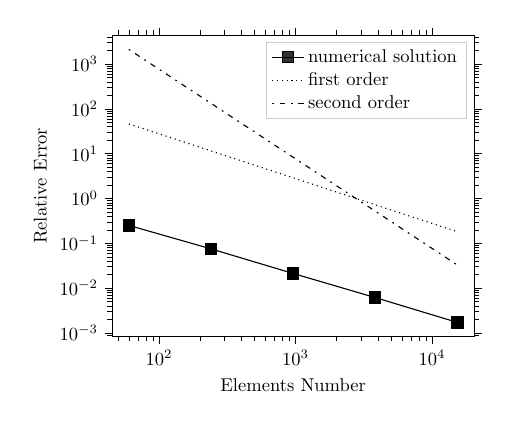
\begin{tikzpicture}[scale=0.67]

\begin{axis}[
legend cell align={left},
legend style={fill opacity=0.8, draw opacity=1, text opacity=1, draw=white!80!black},
log basis x={10},
log basis y={10},
tick align=outside,
tick pos=both,
x grid style={white!69.0196078431373!black},
xlabel={Elements Number},
xmin=45.4714969953119, xmax=20267.6415094717,
xmode=log,
xtick style={color=black},
y grid style={white!69.0196078431373!black},
ylabel={Relative Error},
ymin=0.000842597411085675, ymax=4284.04221578242,
ymode=log,
ytick style={color=black}
]
\addplot [semithick, black, mark=square*, mark size=3, mark options={solid}]
table {%
60 0.249876167836816
240 0.0747309161218632
960 0.0210934232709758
3840 0.00610324223841618
15360 0.0017
};
\addlegendentry{numerical solution}
\addplot [semithick, black, dotted]
table {%
60 46.08
240 11.52
960 2.88
3840 0.72
15360 0.18
};
\addlegendentry{first order}
\addplot [semithick, black, dash pattern=on 1pt off 3pt on 3pt off 3pt]
table {%
60 2123.3664
240 132.7104
960 8.2944
3840 0.5184
15360 0.0324
};
\addlegendentry{second order}
\end{axis}

\end{tikzpicture}

\end{column}

\end{columns}
\end{center}
\end{frame}





%%%%%%%%%%%%%%%%%%%%%%%%%%%%%%%%%%%%%%%%%%%%%%%%%%%%%%%%%%%%%%%%%%%%%%%%%%%%%%%%%%%%%%%%%%


\iffalse
\begin{frame}
 \frametitle{\small Validation - Poiseuille Flow}
\begin{figure}
  \centering
  \vspace{-1.5cm}
  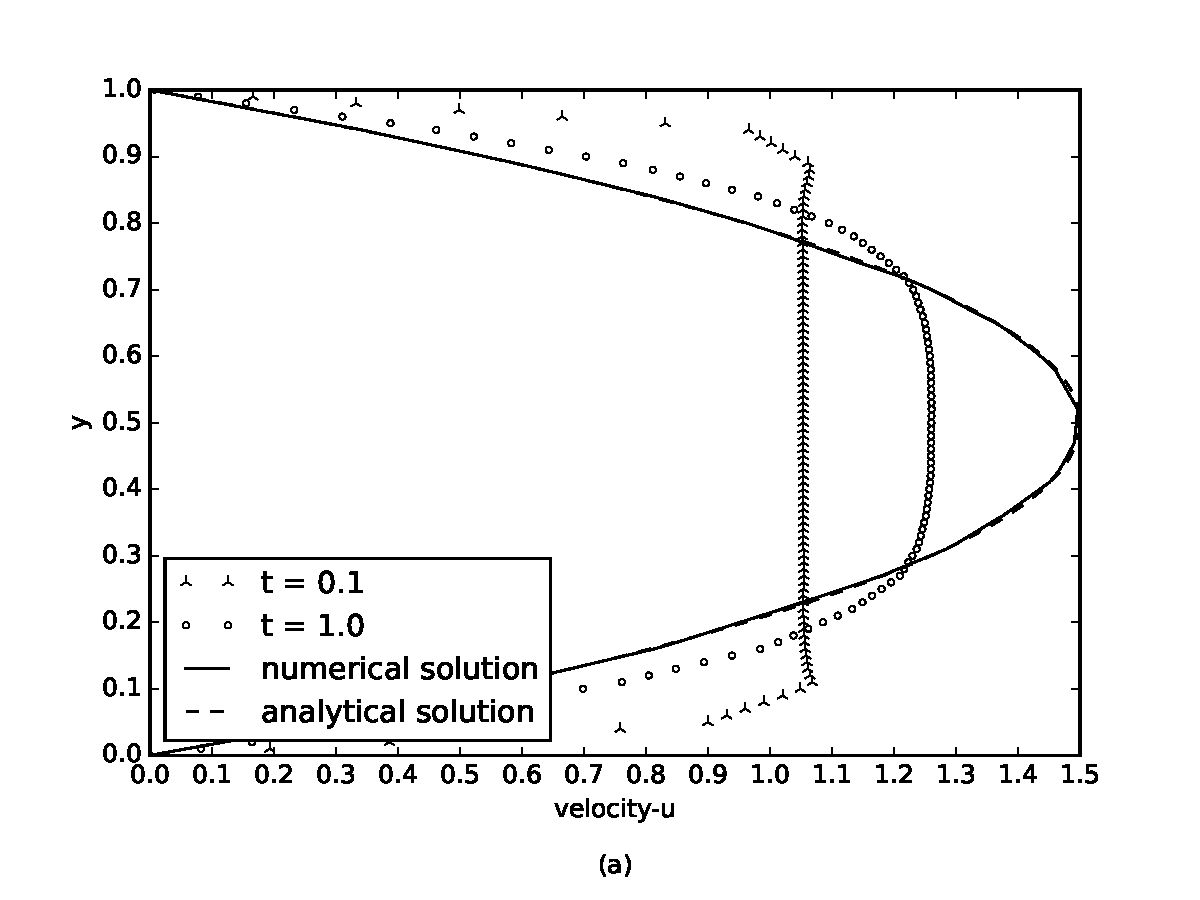
\includegraphics[scale=0.6]{images/poiseuille_velocity.pdf}
\end{figure}
\vspace{-0.2cm}
\centering \scriptsize Evolution of velocity field profile in time for \textit{$Re = 100$} and the comparison between numerical solution and analytical solution.
\end{frame}
\fi

%%%%%%%%%%%%%%%%%%%%%%%%%%%%%%%%%%%%%%%%%%%%%%%%%%%%%%%%%%%%%%%%%%%%%%%%%%%%%%%%%%%%%%%%%%

\begin{frame}
 \frametitle{\LARGE Validation - Lid Driven Cavity Flow}
\vspace{-0.3cm}
\begin{center}
\begin{columns}[c]
\begin{column}{0.65\textwidth} 
\small
Boundaries Conditions:\\[0.2cm]
Bottom and side plates: $u=0$, $v=0$ e $\psi=0$\\[0.1cm]
Top plate: $u=1$, $v=0$ e $\psi=0$\\[0.1cm]
Nodes: 3798\\[0.1cm]
Elements: 7382\\[0.1cm]
Re: 100
\end{column}
\begin{column}{0.25\textwidth} 
\begin{tikzpicture}[scale=0.6]
\draw [pattern=north east lines] (0,-0.1) -- (3,-0.1) -- (3,3) -- (2.9,3) -- (2.9,0) -- (0.1,0) -- (0.1,3) -- (0,3) -- cycle;
 \draw [pattern=north east lines] (-0.1,3) -- (-0.1,3.1) -- (3.1,3.1) -- (3.1,3) -- cycle;

 \draw [->,thick] (3.2,3.05)--(4.2,3.05) node[above] {$U_{top}$};

 \draw [->,thick] (2.4,2.4) arc (45:-180:1.2);

% \draw [->,thick] (-2,-0.1)--(-2,1.5) node[left] {$y$};
% \draw [->,thick] (-2.1,0)--(-0.5,0) node[below] {$x$};
\end{tikzpicture}
\end{column}
\end{columns}
\end{center}

\begin{center}
\begin{columns}[c]
\begin{column}{0.55\textwidth} 
% This file was created by tikzplotlib v0.9.2.
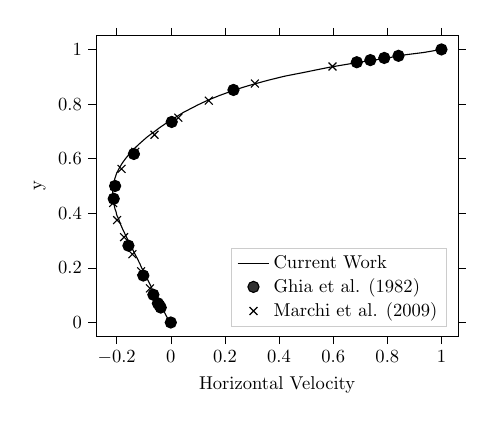
\begin{tikzpicture}[scale=0.67]

\begin{axis}[
legend cell align={left},
legend style={fill opacity=0.8, draw opacity=1, text opacity=1, at={(0.97,0.03)}, anchor=south east, draw=white!80!black},
tick align=outside,
tick pos=both,
x grid style={white!69.0196078431373!black},
xlabel={Horizontal Velocity},
xmin=-0.2751725, xmax=1.0607225,
xtick style={color=black},
y grid style={white!69.0196078431373!black},
ylabel={y},
ymin=-0.05, ymax=1.05,
ytick style={color=black}
]
\addplot [semithick, black]
table {%
0 0
-0.00073216 0.001
-0.0014643 0.002
-0.0021965 0.003
-0.0029286 0.004
-0.0036608 0.005
-0.004393 0.006
-0.0051251 0.007
-0.0058573 0.008
-0.0065894 0.009
-0.0073216 0.01
-0.0080671 0.011
-0.0087826 0.012
-0.0094981 0.013
-0.010214 0.014
-0.010929 0.015
-0.011645 0.016
-0.01236 0.017
-0.013076 0.018
-0.013791 0.019
-0.014507 0.02
-0.015222 0.021
-0.015796 0.022
-0.016279 0.023
-0.016759 0.024
-0.017239 0.025
-0.017719 0.026
-0.018199 0.027
-0.018679 0.028
-0.019159 0.029
-0.019639 0.03
-0.020119 0.031
-0.020599 0.032
-0.021191 0.033
-0.021789 0.034
-0.022386 0.035
-0.022983 0.036
-0.023581 0.037
-0.024178 0.038
-0.024775 0.039
-0.025373 0.04
-0.02597 0.041
-0.026569 0.042
-0.027167 0.043
-0.027765 0.044
-0.028364 0.045
-0.028962 0.046
-0.029561 0.047
-0.030129 0.048
-0.030681 0.049
-0.031232 0.05
-0.031784 0.051
-0.032336 0.052
-0.032888 0.053
-0.03344 0.054
-0.033991 0.055
-0.034535 0.056
-0.035069 0.057
-0.035603 0.058
-0.036137 0.059
-0.036672 0.06
-0.037206 0.061
-0.03774 0.062
-0.038274 0.063
-0.038808 0.064
-0.039342 0.065
-0.039867 0.066
-0.040357 0.067
-0.040847 0.068
-0.041337 0.069
-0.041827 0.07
-0.042317 0.071
-0.042807 0.072
-0.043297 0.073
-0.043787 0.074
-0.044277 0.075
-0.044764 0.076
-0.045249 0.077
-0.045735 0.078
-0.04622 0.079
-0.046706 0.08
-0.047192 0.081
-0.047677 0.082
-0.048163 0.083
-0.048648 0.084
-0.049158 0.085
-0.049734 0.086
-0.050309 0.087
-0.050885 0.088
-0.051461 0.089
-0.052036 0.09
-0.052612 0.091
-0.053187 0.092
-0.053763 0.093
-0.054338 0.094
-0.054914 0.095
-0.055477 0.096
-0.056013 0.097
-0.05655 0.098
-0.057062 0.099
-0.057561 0.1
-0.058061 0.101
-0.058561 0.102
-0.059039 0.103
-0.059509 0.104
-0.059979 0.105
-0.060449 0.106
-0.060919 0.107
-0.061389 0.108
-0.061859 0.109
-0.062329 0.11
-0.062799 0.111
-0.063269 0.112
-0.063771 0.113
-0.064287 0.114
-0.064803 0.115
-0.065319 0.116
-0.065835 0.117
-0.066334 0.118
-0.06683 0.119
-0.067326 0.12
-0.067823 0.121
-0.068319 0.122
-0.068816 0.123
-0.069312 0.124
-0.069809 0.125
-0.070305 0.126
-0.070802 0.127
-0.071294 0.128
-0.071773 0.129
-0.072251 0.13
-0.072729 0.131
-0.073207 0.132
-0.073686 0.133
-0.074164 0.134
-0.074642 0.135
-0.075121 0.136
-0.075599 0.137
-0.076077 0.138
-0.076555 0.139
-0.077023 0.14
-0.077488 0.141
-0.077953 0.142
-0.078418 0.143
-0.078883 0.144
-0.07939 0.145
-0.079916 0.146
-0.080442 0.147
-0.080968 0.148
-0.081495 0.149
-0.082021 0.15
-0.082547 0.151
-0.083073 0.152
-0.083599 0.153
-0.084125 0.154
-0.084651 0.155
-0.085178 0.156
-0.085704 0.157
-0.08623 0.158
-0.086717 0.159
-0.087187 0.16
-0.087658 0.161
-0.088131 0.162
-0.088605 0.163
-0.089078 0.164
-0.089552 0.165
-0.090025 0.166
-0.090499 0.167
-0.090973 0.168
-0.091446 0.169
-0.09192 0.17
-0.092393 0.171
-0.092867 0.172
-0.09334 0.173
-0.093814 0.174
-0.094287 0.175
-0.094761 0.176
-0.095236 0.177
-0.095716 0.178
-0.096195 0.179
-0.096675 0.18
-0.097155 0.181
-0.097635 0.182
-0.098115 0.183
-0.098595 0.184
-0.099075 0.185
-0.099555 0.186
-0.10003 0.187
-0.10051 0.188
-0.10099 0.189
-0.1015 0.19
-0.10212 0.191
-0.10274 0.192
-0.10336 0.193
-0.10397 0.194
-0.10459 0.195
-0.10521 0.196
-0.10583 0.197
-0.10644 0.198
-0.10706 0.199
-0.10768 0.2
-0.10824 0.201
-0.10867 0.202
-0.10908 0.203
-0.10949 0.204
-0.10991 0.205
-0.11032 0.206
-0.11073 0.207
-0.11114 0.208
-0.11155 0.209
-0.11196 0.21
-0.11237 0.211
-0.11279 0.212
-0.1132 0.213
-0.11361 0.214
-0.11408 0.215
-0.11466 0.216
-0.11524 0.217
-0.11577 0.218
-0.11626 0.219
-0.11676 0.22
-0.11726 0.221
-0.11775 0.222
-0.11825 0.223
-0.11875 0.224
-0.11924 0.225
-0.11974 0.226
-0.12024 0.227
-0.12073 0.228
-0.12123 0.229
-0.12173 0.23
-0.12223 0.231
-0.12273 0.232
-0.12323 0.233
-0.12372 0.234
-0.12421 0.235
-0.12473 0.236
-0.12526 0.237
-0.1258 0.238
-0.12634 0.239
-0.12688 0.24
-0.12741 0.241
-0.12795 0.242
-0.12849 0.243
-0.12903 0.244
-0.12956 0.245
-0.1301 0.246
-0.13064 0.247
-0.13118 0.248
-0.13171 0.249
-0.13223 0.25
-0.13275 0.251
-0.13326 0.252
-0.13377 0.253
-0.13426 0.254
-0.13476 0.255
-0.13526 0.256
-0.13575 0.257
-0.13625 0.258
-0.13674 0.259
-0.13724 0.26
-0.13774 0.261
-0.13823 0.262
-0.13876 0.263
-0.13929 0.264
-0.13981 0.265
-0.14034 0.266
-0.14087 0.267
-0.1414 0.268
-0.14191 0.269
-0.1424 0.27
-0.1429 0.271
-0.14339 0.272
-0.14389 0.273
-0.14438 0.274
-0.14488 0.275
-0.14538 0.276
-0.14587 0.277
-0.14635 0.278
-0.14683 0.279
-0.14732 0.28
-0.1478 0.281
-0.14828 0.282
-0.14876 0.283
-0.14925 0.284
-0.14973 0.285
-0.15021 0.286
-0.15069 0.287
-0.15118 0.288
-0.15166 0.289
-0.15214 0.29
-0.15262 0.291
-0.15311 0.292
-0.15361 0.293
-0.15411 0.294
-0.15462 0.295
-0.15512 0.296
-0.15562 0.297
-0.15613 0.298
-0.15663 0.299
-0.15714 0.3
-0.15764 0.301
-0.15814 0.302
-0.15865 0.303
-0.15915 0.304
-0.15965 0.305
-0.16016 0.306
-0.16066 0.307
-0.16118 0.308
-0.16169 0.309
-0.1622 0.31
-0.16272 0.311
-0.16323 0.312
-0.16375 0.313
-0.16426 0.314
-0.16477 0.315
-0.16528 0.316
-0.16578 0.317
-0.16627 0.318
-0.16676 0.319
-0.16726 0.32
-0.16775 0.321
-0.16824 0.322
-0.16873 0.323
-0.16923 0.324
-0.16972 0.325
-0.17022 0.326
-0.17071 0.327
-0.1712 0.328
-0.1717 0.329
-0.17219 0.33
-0.17269 0.331
-0.17318 0.332
-0.17367 0.333
-0.17417 0.334
-0.17466 0.335
-0.17516 0.336
-0.17565 0.337
-0.17614 0.338
-0.17664 0.339
-0.1771 0.34
-0.17754 0.341
-0.17798 0.342
-0.17842 0.343
-0.17886 0.344
-0.17929 0.345
-0.17973 0.346
-0.18017 0.347
-0.18061 0.348
-0.18105 0.349
-0.18149 0.35
-0.18193 0.351
-0.18237 0.352
-0.1828 0.353
-0.18324 0.354
-0.18368 0.355
-0.18412 0.356
-0.18456 0.357
-0.18499 0.358
-0.18542 0.359
-0.18585 0.36
-0.18627 0.361
-0.18666 0.362
-0.18701 0.363
-0.18735 0.364
-0.18769 0.365
-0.18803 0.366
-0.18837 0.367
-0.18872 0.368
-0.18906 0.369
-0.1894 0.37
-0.18974 0.371
-0.19009 0.372
-0.19043 0.373
-0.19077 0.374
-0.19111 0.375
-0.19145 0.376
-0.1918 0.377
-0.19224 0.378
-0.19269 0.379
-0.19316 0.38
-0.19364 0.381
-0.19412 0.382
-0.19461 0.383
-0.19509 0.384
-0.19558 0.385
-0.19606 0.386
-0.19654 0.387
-0.19703 0.388
-0.19751 0.389
-0.198 0.39
-0.19848 0.391
-0.19896 0.392
-0.19936 0.393
-0.19967 0.394
-0.19997 0.395
-0.20028 0.396
-0.20059 0.397
-0.20079 0.398
-0.20099 0.399
-0.20119 0.4
-0.20139 0.401
-0.20159 0.402
-0.20179 0.403
-0.20199 0.404
-0.20219 0.405
-0.20239 0.406
-0.20275 0.407
-0.20318 0.408
-0.20361 0.409
-0.20403 0.41
-0.20446 0.411
-0.20489 0.412
-0.20532 0.413
-0.20564 0.414
-0.20589 0.415
-0.20614 0.416
-0.2064 0.417
-0.20665 0.418
-0.20691 0.419
-0.20716 0.42
-0.20742 0.421
-0.20763 0.422
-0.20783 0.423
-0.20803 0.424
-0.20824 0.425
-0.20844 0.426
-0.20864 0.427
-0.20884 0.428
-0.20905 0.429
-0.20925 0.43
-0.20945 0.431
-0.20965 0.432
-0.20985 0.433
-0.21006 0.434
-0.21033 0.435
-0.2105 0.436
-0.21067 0.437
-0.21084 0.438
-0.21101 0.439
-0.21118 0.44
-0.21135 0.441
-0.21152 0.442
-0.21169 0.443
-0.21185 0.444
-0.21202 0.445
-0.21219 0.446
-0.21236 0.447
-0.21253 0.448
-0.2127 0.449
-0.21287 0.45
-0.21302 0.451
-0.2131 0.452
-0.21318 0.453
-0.21325 0.454
-0.2133 0.455
-0.21335 0.456
-0.2134 0.457
-0.21345 0.458
-0.21351 0.459
-0.21356 0.46
-0.21363 0.461
-0.2137 0.462
-0.21377 0.463
-0.21384 0.464
-0.21391 0.465
-0.21398 0.466
-0.21405 0.467
-0.21412 0.468
-0.21416 0.469
-0.21418 0.47
-0.21421 0.471
-0.21424 0.472
-0.21427 0.473
-0.21429 0.474
-0.21432 0.475
-0.21435 0.476
-0.21438 0.477
-0.2144 0.478
-0.21443 0.479
-0.21445 0.48
-0.21445 0.481
-0.21445 0.482
-0.21444 0.483
-0.21436 0.484
-0.21428 0.485
-0.2142 0.486
-0.21412 0.487
-0.21404 0.488
-0.21396 0.489
-0.21388 0.49
-0.2138 0.491
-0.21372 0.492
-0.21364 0.493
-0.21356 0.494
-0.21348 0.495
-0.2134 0.496
-0.21332 0.497
-0.21324 0.498
-0.21309 0.499
-0.21293 0.5
-0.21275 0.501
-0.21258 0.502
-0.2124 0.503
-0.21223 0.504
-0.21205 0.505
-0.21188 0.506
-0.2117 0.507
-0.21152 0.508
-0.21135 0.509
-0.21117 0.51
-0.211 0.511
-0.21082 0.512
-0.21065 0.513
-0.21046 0.514
-0.21021 0.515
-0.20995 0.516
-0.2097 0.517
-0.20944 0.518
-0.20913 0.519
-0.20882 0.52
-0.20851 0.521
-0.2082 0.522
-0.20788 0.523
-0.20757 0.524
-0.20726 0.525
-0.20695 0.526
-0.20664 0.527
-0.20633 0.528
-0.20602 0.529
-0.2057 0.53
-0.20537 0.531
-0.20503 0.532
-0.2047 0.533
-0.20437 0.534
-0.20403 0.535
-0.2037 0.536
-0.20337 0.537
-0.20303 0.538
-0.2027 0.539
-0.20236 0.54
-0.20203 0.541
-0.20169 0.542
-0.20136 0.543
-0.20103 0.544
-0.20069 0.545
-0.20036 0.546
-0.20002 0.547
-0.19953 0.548
-0.199 0.549
-0.19848 0.55
-0.19796 0.551
-0.19744 0.552
-0.19692 0.553
-0.19639 0.554
-0.19587 0.555
-0.19535 0.556
-0.19483 0.557
-0.1943 0.558
-0.19378 0.559
-0.19326 0.56
-0.19274 0.561
-0.19221 0.562
-0.19169 0.563
-0.19117 0.564
-0.19064 0.565
-0.19012 0.566
-0.18956 0.567
-0.18901 0.568
-0.18845 0.569
-0.18788 0.57
-0.18725 0.571
-0.18661 0.572
-0.18597 0.573
-0.18534 0.574
-0.1847 0.575
-0.18407 0.576
-0.18343 0.577
-0.1828 0.578
-0.18216 0.579
-0.18153 0.58
-0.18089 0.581
-0.18026 0.582
-0.17962 0.583
-0.17899 0.584
-0.17834 0.585
-0.17762 0.586
-0.1769 0.587
-0.17619 0.588
-0.17547 0.589
-0.17475 0.59
-0.17402 0.591
-0.17328 0.592
-0.17254 0.593
-0.1718 0.594
-0.17106 0.595
-0.17032 0.596
-0.16958 0.597
-0.16884 0.598
-0.16809 0.599
-0.1673 0.6
-0.16651 0.601
-0.16572 0.602
-0.16493 0.603
-0.16414 0.604
-0.16335 0.605
-0.16256 0.606
-0.16173 0.607
-0.16082 0.608
-0.15991 0.609
-0.159 0.61
-0.1581 0.611
-0.15719 0.612
-0.15628 0.613
-0.15537 0.614
-0.15447 0.615
-0.15359 0.616
-0.1527 0.617
-0.15181 0.618
-0.15092 0.619
-0.15004 0.62
-0.14915 0.621
-0.14826 0.622
-0.14737 0.623
-0.14646 0.624
-0.14555 0.625
-0.14464 0.626
-0.14373 0.627
-0.14282 0.628
-0.14191 0.629
-0.14098 0.63
-0.14005 0.631
-0.13912 0.632
-0.13818 0.633
-0.13725 0.634
-0.13632 0.635
-0.13539 0.636
-0.13446 0.637
-0.13353 0.638
-0.13247 0.639
-0.13142 0.64
-0.13037 0.641
-0.12931 0.642
-0.12826 0.643
-0.1272 0.644
-0.12615 0.645
-0.1251 0.646
-0.12404 0.647
-0.12299 0.648
-0.12194 0.649
-0.12088 0.65
-0.11983 0.651
-0.11875 0.652
-0.11762 0.653
-0.11649 0.654
-0.11536 0.655
-0.11422 0.656
-0.11308 0.657
-0.11194 0.658
-0.11081 0.659
-0.10967 0.66
-0.10853 0.661
-0.10739 0.662
-0.10625 0.663
-0.10511 0.664
-0.10397 0.665
-0.10283 0.666
-0.10169 0.667
-0.10055 0.668
-0.099406 0.669
-0.098265 0.67
-0.097125 0.671
-0.095984 0.672
-0.094844 0.673
-0.0937 0.674
-0.092501 0.675
-0.091302 0.676
-0.090103 0.677
-0.088903 0.678
-0.087704 0.679
-0.086449 0.68
-0.085122 0.681
-0.083796 0.682
-0.082469 0.683
-0.081143 0.684
-0.079817 0.685
-0.07849 0.686
-0.077164 0.687
-0.075837 0.688
-0.074511 0.689
-0.073184 0.69
-0.071804 0.691
-0.070401 0.692
-0.068997 0.693
-0.067594 0.694
-0.066191 0.695
-0.064788 0.696
-0.063384 0.697
-0.061981 0.698
-0.060578 0.699
-0.059257 0.7
-0.057942 0.701
-0.056626 0.702
-0.055311 0.703
-0.053995 0.704
-0.05268 0.705
-0.051348 0.706
-0.050014 0.707
-0.048681 0.708
-0.047348 0.709
-0.046015 0.71
-0.044681 0.711
-0.043348 0.712
-0.041947 0.713
-0.040468 0.714
-0.038988 0.715
-0.037509 0.716
-0.03603 0.717
-0.034551 0.718
-0.033072 0.719
-0.031593 0.72
-0.030114 0.721
-0.028635 0.722
-0.027164 0.723
-0.025739 0.724
-0.024315 0.725
-0.02289 0.726
-0.021459 0.727
-0.019976 0.728
-0.018493 0.729
-0.017005 0.73
-0.015489 0.731
-0.013973 0.732
-0.012457 0.733
-0.010941 0.734
-0.0094249 0.735
-0.007909 0.736
-0.0063931 0.737
-0.0048771 0.738
-0.0033611 0.739
-0.0018452 0.74
-0.00018525 0.741
0.0014945 0.742
0.0031742 0.743
0.0048541 0.744
0.0065338 0.745
0.0082135 0.746
0.0098933 0.747
0.011573 0.748
0.013253 0.749
0.014949 0.75
0.016663 0.751
0.018377 0.752
0.020092 0.753
0.021763 0.754
0.023369 0.755
0.024976 0.756
0.026582 0.757
0.028189 0.758
0.029795 0.759
0.031402 0.76
0.033008 0.761
0.034615 0.762
0.036221 0.763
0.037828 0.764
0.039434 0.765
0.041041 0.766
0.042638 0.767
0.044215 0.768
0.045896 0.769
0.047824 0.77
0.049764 0.771
0.051704 0.772
0.053645 0.773
0.055585 0.774
0.057525 0.775
0.059465 0.776
0.061406 0.777
0.063346 0.778
0.065286 0.779
0.067226 0.78
0.069167 0.781
0.071107 0.782
0.073047 0.783
0.074915 0.784
0.076762 0.785
0.078689 0.786
0.080665 0.787
0.082641 0.788
0.084618 0.789
0.086594 0.79
0.08857 0.791
0.090547 0.792
0.092523 0.793
0.094499 0.794
0.096475 0.795
0.098452 0.796
0.10044 0.797
0.10253 0.798
0.10462 0.799
0.10672 0.8
0.10881 0.801
0.1109 0.802
0.113 0.803
0.11509 0.804
0.11721 0.805
0.11944 0.806
0.12168 0.807
0.12391 0.808
0.12615 0.809
0.12838 0.81
0.13062 0.811
0.13286 0.812
0.13509 0.813
0.13733 0.814
0.13956 0.815
0.14187 0.816
0.14436 0.817
0.14685 0.818
0.14934 0.819
0.15182 0.82
0.15431 0.821
0.1568 0.822
0.15929 0.823
0.16178 0.824
0.16426 0.825
0.16675 0.826
0.16924 0.827
0.17173 0.828
0.17421 0.829
0.1767 0.83
0.17918 0.831
0.18182 0.832
0.18461 0.833
0.18741 0.834
0.1902 0.835
0.193 0.836
0.1958 0.837
0.19859 0.838
0.20139 0.839
0.20418 0.84
0.20698 0.841
0.20977 0.842
0.21257 0.843
0.21536 0.844
0.21816 0.845
0.22095 0.846
0.22381 0.847
0.22675 0.848
0.2297 0.849
0.23264 0.85
0.23559 0.851
0.23853 0.852
0.24155 0.853
0.24464 0.854
0.24772 0.855
0.25081 0.856
0.25389 0.857
0.25697 0.858
0.26006 0.859
0.26314 0.86
0.26622 0.861
0.26931 0.862
0.27252 0.863
0.27595 0.864
0.27939 0.865
0.28283 0.866
0.28626 0.867
0.2897 0.868
0.29314 0.869
0.29657 0.87
0.30001 0.871
0.30367 0.872
0.30734 0.873
0.31101 0.874
0.31468 0.875
0.31835 0.876
0.32202 0.877
0.3257 0.878
0.32937 0.879
0.33304 0.88
0.33671 0.881
0.34038 0.882
0.34405 0.883
0.34786 0.884
0.35171 0.885
0.35557 0.886
0.35942 0.887
0.36343 0.888
0.36747 0.889
0.37151 0.89
0.37555 0.891
0.37959 0.892
0.38363 0.893
0.38767 0.894
0.39171 0.895
0.39575 0.896
0.39985 0.897
0.40401 0.898
0.40816 0.899
0.41232 0.9
0.41648 0.901
0.42101 0.902
0.42593 0.903
0.43085 0.904
0.4359 0.905
0.44109 0.906
0.44629 0.907
0.45148 0.908
0.45667 0.909
0.46187 0.91
0.46706 0.911
0.47225 0.912
0.47745 0.913
0.48264 0.914
0.48784 0.915
0.49285 0.916
0.49781 0.917
0.50276 0.918
0.50772 0.919
0.51267 0.92
0.51763 0.921
0.52259 0.922
0.52754 0.923
0.5325 0.924
0.53747 0.925
0.54247 0.926
0.54747 0.927
0.55248 0.928
0.55748 0.929
0.56249 0.93
0.56749 0.931
0.57249 0.932
0.5775 0.933
0.5825 0.934
0.58822 0.935
0.59411 0.936
0.60001 0.937
0.60591 0.938
0.6118 0.939
0.6177 0.94
0.6236 0.941
0.62949 0.942
0.63539 0.943
0.64128 0.944
0.64729 0.945
0.65338 0.946
0.65947 0.947
0.66556 0.948
0.67164 0.949
0.67773 0.95
0.68382 0.951
0.68991 0.952
0.69631 0.953
0.70325 0.954
0.7102 0.955
0.71714 0.956
0.72409 0.957
0.73103 0.958
0.73798 0.959
0.74467 0.96
0.75133 0.961
0.75798 0.962
0.76464 0.963
0.77129 0.964
0.77795 0.965
0.7846 0.966
0.79126 0.967
0.79784 0.968
0.80301 0.969
0.80818 0.97
0.81335 0.971
0.81852 0.972
0.82369 0.973
0.82886 0.974
0.83403 0.975
0.8392 0.976
0.84437 0.977
0.84959 0.978
0.85612 0.979
0.86408 0.98
0.87205 0.981
0.88001 0.982
0.88797 0.983
0.89594 0.984
0.9039 0.985
0.91187 0.986
0.91983 0.987
0.92779 0.988
0.93576 0.989
0.94175 0.99
0.94758 0.991
0.9534 0.992
0.95922 0.993
0.96505 0.994
0.97088 0.995
0.9767 0.996
0.98252 0.997
0.98835 0.998
0.99418 0.999
1 1
};
\addlegendentry{Current Work}
\addplot [semithick, black, mark=*, mark size=3, mark options={solid}, only marks]
table {%
0 0
-0.03717 0.0547
-0.04192 0.0625
-0.04775 0.0703
-0.06434 0.1016
-0.1015 0.1719
-0.15662 0.2813
-0.2109 0.4531
-0.20581 0.5
-0.13641 0.6172
0.00332 0.7344
0.23151 0.8516
0.68717 0.9531
0.73722 0.9609
0.78871 0.9688
0.84123 0.9766
1 1
};
\addlegendentry{Ghia et al. (1982)}
\addplot [semithick, black, mark=x, mark size=3, mark options={solid}, only marks]
table {%
0 0
-0.04197 0.0625
-0.07712 0.125
-0.10981 0.1875
-0.14193 0.25
-0.17271 0.3125
-0.19847 0.375
-0.21296 0.4375
-0.20914 0.5
-0.18208 0.5625
-0.13125 0.625
-0.06024 0.6875
0.02787 0.75
0.14042 0.8125
0.31055 0.875
0.59746 0.9375
1 1
};
\addlegendentry{Marchi et al. (2009)}
\end{axis}

\end{tikzpicture}

\end{column}

\begin{column}{0.55\textwidth} 
\hspace{0.5cm}
% This file was created by tikzplotlib v0.9.2.
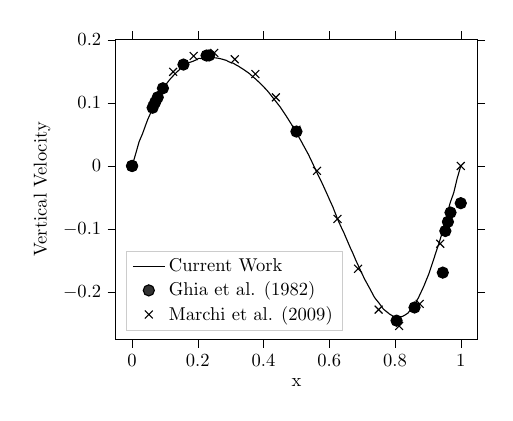
\begin{tikzpicture}[scale=0.67]

\begin{axis}[
legend cell align={left},
legend style={fill opacity=0.8, draw opacity=1, text opacity=1, at={(0.03,0.03)}, anchor=south west, draw=white!80!black},
tick align=outside,
tick pos=both,
x grid style={white!69.0196078431373!black},
xlabel={x},
xmin=-0.05, xmax=1.05,
xtick style={color=black},
y grid style={white!69.0196078431373!black},
ylabel={Vertical Velocity},
ymin=-0.27541, ymax=0.20089,
ytick style={color=black}
]
\addplot [semithick, black]
table {%
0 0
0.001 0.0017478
0.002 0.0034956
0.003 0.0052434
0.004 0.0069911
0.005 0.0087389
0.006 0.010487
0.007 0.012235
0.008 0.013982
0.009 0.01573
0.01 0.017478
0.011 0.019311
0.012 0.02115
0.013 0.022988
0.014 0.024826
0.015 0.026665
0.016 0.028503
0.017 0.030341
0.018 0.032179
0.019 0.034018
0.02 0.035856
0.021 0.037694
0.022 0.039222
0.023 0.040449
0.024 0.041665
0.025 0.042881
0.026 0.044096
0.027 0.045312
0.028 0.046527
0.029 0.047743
0.03 0.048958
0.031 0.050174
0.032 0.051389
0.033 0.052825
0.034 0.054271
0.035 0.055717
0.036 0.057163
0.037 0.058609
0.038 0.060056
0.039 0.061502
0.04 0.062948
0.041 0.064388
0.042 0.065794
0.043 0.0672
0.044 0.068606
0.045 0.070012
0.046 0.071418
0.047 0.072824
0.048 0.074075
0.049 0.07524
0.05 0.076406
0.051 0.077572
0.052 0.078737
0.053 0.079903
0.054 0.081069
0.055 0.082234
0.056 0.083414
0.057 0.084612
0.058 0.085809
0.059 0.087006
0.06 0.088203
0.061 0.0894
0.062 0.090598
0.063 0.091795
0.064 0.092992
0.065 0.094189
0.066 0.095331
0.067 0.09626
0.068 0.097188
0.069 0.098117
0.07 0.099045
0.071 0.099974
0.072 0.1009
0.073 0.10183
0.074 0.10276
0.075 0.10369
0.076 0.10458
0.077 0.10547
0.078 0.10636
0.079 0.10724
0.08 0.10813
0.081 0.10901
0.082 0.1099
0.083 0.11078
0.084 0.11167
0.085 0.11258
0.086 0.11357
0.087 0.11456
0.088 0.11556
0.089 0.11655
0.09 0.11754
0.091 0.11853
0.092 0.11952
0.093 0.12051
0.094 0.12151
0.095 0.1225
0.096 0.12346
0.097 0.12439
0.098 0.12533
0.099 0.12616
0.1 0.12691
0.101 0.12765
0.102 0.12839
0.103 0.12914
0.104 0.12985
0.105 0.13052
0.106 0.13119
0.107 0.13187
0.108 0.13254
0.109 0.13322
0.11 0.13389
0.111 0.13456
0.112 0.13524
0.113 0.13591
0.114 0.13656
0.115 0.13721
0.116 0.13786
0.117 0.13849
0.118 0.13904
0.119 0.1396
0.12 0.14016
0.121 0.14071
0.122 0.14127
0.123 0.14182
0.124 0.14238
0.125 0.14294
0.126 0.14349
0.127 0.14405
0.128 0.1446
0.129 0.14516
0.13 0.14567
0.131 0.14619
0.132 0.14671
0.133 0.14722
0.134 0.14774
0.135 0.14825
0.136 0.14877
0.137 0.14928
0.138 0.14978
0.139 0.15026
0.14 0.15074
0.141 0.15121
0.142 0.15169
0.143 0.15217
0.144 0.15265
0.145 0.15313
0.146 0.15361
0.147 0.15409
0.148 0.15453
0.149 0.15493
0.15 0.15532
0.151 0.15572
0.152 0.15611
0.153 0.15651
0.154 0.15692
0.155 0.15735
0.156 0.15777
0.157 0.1582
0.158 0.15862
0.159 0.15905
0.16 0.15947
0.161 0.1599
0.162 0.16032
0.163 0.16075
0.164 0.16117
0.165 0.1616
0.166 0.16202
0.167 0.16245
0.168 0.16287
0.169 0.16323
0.17 0.16341
0.171 0.16357
0.172 0.16374
0.173 0.1639
0.174 0.16407
0.175 0.16423
0.176 0.16439
0.177 0.16456
0.178 0.16472
0.179 0.16489
0.18 0.16505
0.181 0.16522
0.182 0.16538
0.183 0.16555
0.184 0.16571
0.185 0.16592
0.186 0.16615
0.187 0.16638
0.188 0.16662
0.189 0.16685
0.19 0.16708
0.191 0.16731
0.192 0.16754
0.193 0.16777
0.194 0.168
0.195 0.16824
0.196 0.16853
0.197 0.16883
0.198 0.16914
0.199 0.16944
0.2 0.16975
0.201 0.17005
0.202 0.17036
0.203 0.17066
0.204 0.17063
0.205 0.17058
0.206 0.17053
0.207 0.17049
0.208 0.17044
0.209 0.1704
0.21 0.17035
0.211 0.1703
0.212 0.17026
0.213 0.17021
0.214 0.17017
0.215 0.17021
0.216 0.17028
0.217 0.17036
0.218 0.17049
0.219 0.17062
0.22 0.17075
0.221 0.17088
0.222 0.17101
0.223 0.17114
0.224 0.17127
0.225 0.1714
0.226 0.17153
0.227 0.17165
0.228 0.17178
0.229 0.17191
0.23 0.17204
0.231 0.17211
0.232 0.17209
0.233 0.17209
0.234 0.17208
0.235 0.17207
0.236 0.17205
0.237 0.17202
0.238 0.172
0.239 0.17198
0.24 0.17196
0.241 0.17193
0.242 0.17191
0.243 0.17189
0.244 0.17187
0.245 0.17184
0.246 0.17182
0.247 0.17177
0.248 0.1717
0.249 0.17163
0.25 0.17156
0.251 0.17151
0.252 0.17145
0.253 0.17139
0.254 0.17133
0.255 0.17128
0.256 0.17122
0.257 0.17116
0.258 0.1711
0.259 0.17105
0.26 0.17097
0.261 0.17087
0.262 0.17077
0.263 0.17066
0.264 0.17056
0.265 0.17046
0.266 0.17036
0.267 0.17025
0.268 0.17015
0.269 0.17005
0.27 0.16994
0.271 0.16976
0.272 0.16958
0.273 0.1694
0.274 0.16929
0.275 0.16918
0.276 0.16907
0.277 0.16891
0.278 0.16875
0.279 0.16859
0.28 0.16844
0.281 0.16828
0.282 0.16812
0.283 0.16796
0.284 0.1678
0.285 0.16764
0.286 0.16749
0.287 0.1673
0.288 0.16703
0.289 0.16676
0.29 0.16648
0.291 0.16621
0.292 0.16594
0.293 0.16567
0.294 0.1654
0.295 0.16515
0.296 0.16491
0.297 0.16467
0.298 0.16443
0.299 0.16419
0.3 0.16396
0.301 0.16383
0.302 0.16369
0.303 0.16355
0.304 0.16341
0.305 0.16327
0.306 0.16313
0.307 0.16299
0.308 0.16285
0.309 0.16254
0.31 0.16222
0.311 0.1619
0.312 0.16158
0.313 0.16126
0.314 0.16094
0.315 0.16063
0.316 0.16031
0.317 0.15999
0.318 0.15967
0.319 0.15941
0.32 0.15916
0.321 0.15891
0.322 0.15866
0.323 0.1584
0.324 0.15806
0.325 0.15772
0.326 0.15738
0.327 0.15704
0.328 0.1567
0.329 0.15636
0.33 0.15601
0.331 0.15567
0.332 0.15533
0.333 0.155
0.334 0.15467
0.335 0.15435
0.336 0.15403
0.337 0.1537
0.338 0.15338
0.339 0.15305
0.34 0.15269
0.341 0.15232
0.342 0.15195
0.343 0.15159
0.344 0.15123
0.345 0.15086
0.346 0.1505
0.347 0.15014
0.348 0.14978
0.349 0.14942
0.35 0.14906
0.351 0.14869
0.352 0.14833
0.353 0.14797
0.354 0.14761
0.355 0.14725
0.356 0.14687
0.357 0.14641
0.358 0.14594
0.359 0.14548
0.36 0.14502
0.361 0.14455
0.362 0.14409
0.363 0.14362
0.364 0.14316
0.365 0.14269
0.366 0.14223
0.367 0.14176
0.368 0.1413
0.369 0.14085
0.37 0.14042
0.371 0.13999
0.372 0.13955
0.373 0.13912
0.374 0.13867
0.375 0.13819
0.376 0.13772
0.377 0.13724
0.378 0.13676
0.379 0.13628
0.38 0.1358
0.381 0.13532
0.382 0.13484
0.383 0.13437
0.384 0.13389
0.385 0.13341
0.386 0.13293
0.387 0.13245
0.388 0.13197
0.389 0.13149
0.39 0.13102
0.391 0.13048
0.392 0.12994
0.393 0.12941
0.394 0.12887
0.395 0.12834
0.396 0.1278
0.397 0.12727
0.398 0.12674
0.399 0.1262
0.4 0.12566
0.401 0.1251
0.402 0.12455
0.403 0.124
0.404 0.12345
0.405 0.12289
0.406 0.12234
0.407 0.12179
0.408 0.12124
0.409 0.12068
0.41 0.12013
0.411 0.11956
0.412 0.11894
0.413 0.11831
0.414 0.11768
0.415 0.11706
0.416 0.11643
0.417 0.11578
0.418 0.11512
0.419 0.11446
0.42 0.1138
0.421 0.11314
0.422 0.11248
0.423 0.11182
0.424 0.11116
0.425 0.1105
0.426 0.10983
0.427 0.10917
0.428 0.10851
0.429 0.10785
0.43 0.10719
0.431 0.10653
0.432 0.10586
0.433 0.1052
0.434 0.10454
0.435 0.10388
0.436 0.10322
0.437 0.10255
0.438 0.10189
0.439 0.10123
0.44 0.10057
0.441 0.099905
0.442 0.099242
0.443 0.09858
0.444 0.097918
0.445 0.097255
0.446 0.096593
0.447 0.095931
0.448 0.095268
0.449 0.094606
0.45 0.093944
0.451 0.093268
0.452 0.092483
0.453 0.091696
0.454 0.09091
0.455 0.090123
0.456 0.089337
0.457 0.08855
0.458 0.087764
0.459 0.086978
0.46 0.086191
0.461 0.085405
0.462 0.084618
0.463 0.083832
0.464 0.083045
0.465 0.082259
0.466 0.081472
0.467 0.080686
0.468 0.079887
0.469 0.079074
0.47 0.078262
0.471 0.077449
0.472 0.076636
0.473 0.075823
0.474 0.07501
0.475 0.074196
0.476 0.073369
0.477 0.072541
0.478 0.071714
0.479 0.070887
0.48 0.070059
0.481 0.069232
0.482 0.068404
0.483 0.067577
0.484 0.066749
0.485 0.065874
0.486 0.064999
0.487 0.064125
0.488 0.06325
0.489 0.062375
0.49 0.061501
0.491 0.060626
0.492 0.059751
0.493 0.058877
0.494 0.058002
0.495 0.057127
0.496 0.056253
0.497 0.055378
0.498 0.054501
0.499 0.053614
0.5 0.052727
0.501 0.051787
0.502 0.050848
0.503 0.049909
0.504 0.048969
0.505 0.04803
0.506 0.047096
0.507 0.046168
0.508 0.045241
0.509 0.044314
0.51 0.043386
0.511 0.042459
0.512 0.041532
0.513 0.040605
0.514 0.039677
0.515 0.03875
0.516 0.037807
0.517 0.036804
0.518 0.0358
0.519 0.034797
0.52 0.03384
0.521 0.032892
0.522 0.031943
0.523 0.030995
0.524 0.030047
0.525 0.029099
0.526 0.02815
0.527 0.027202
0.528 0.026254
0.529 0.025306
0.53 0.024357
0.531 0.023409
0.532 0.02246
0.533 0.021509
0.534 0.020557
0.535 0.019605
0.536 0.018653
0.537 0.017599
0.538 0.016507
0.539 0.015415
0.54 0.014323
0.541 0.013231
0.542 0.012139
0.543 0.011047
0.544 0.0099552
0.545 0.0088633
0.546 0.0077714
0.547 0.0066795
0.548 0.0055849
0.549 0.0044685
0.55 0.0033521
0.551 0.0022358
0.552 0.0011195
0.553 3.1308e-06
0.554 -0.0011133
0.555 -0.0022296
0.556 -0.0033459
0.557 -0.0044623
0.558 -0.0055787
0.559 -0.0066959
0.56 -0.0078154
0.561 -0.0089348
0.562 -0.010054
0.563 -0.0112
0.564 -0.01236
0.565 -0.01352
0.566 -0.014586
0.567 -0.015638
0.568 -0.016691
0.569 -0.017744
0.57 -0.018796
0.571 -0.019849
0.572 -0.020902
0.573 -0.021955
0.574 -0.023007
0.575 -0.02406
0.576 -0.025113
0.577 -0.026165
0.578 -0.027232
0.579 -0.028366
0.58 -0.029501
0.581 -0.030635
0.582 -0.03177
0.583 -0.032905
0.584 -0.034039
0.585 -0.035174
0.586 -0.036308
0.587 -0.037443
0.588 -0.03859
0.589 -0.039745
0.59 -0.0409
0.591 -0.042054
0.592 -0.043209
0.593 -0.044364
0.594 -0.045518
0.595 -0.046676
0.596 -0.04786
0.597 -0.049044
0.598 -0.050227
0.599 -0.051411
0.6 -0.052595
0.601 -0.053779
0.602 -0.054962
0.603 -0.056094
0.604 -0.05722
0.605 -0.058346
0.606 -0.059472
0.607 -0.060597
0.608 -0.061723
0.609 -0.062849
0.61 -0.063978
0.611 -0.065293
0.612 -0.066609
0.613 -0.067924
0.614 -0.06924
0.615 -0.070556
0.616 -0.071871
0.617 -0.073187
0.618 -0.074502
0.619 -0.075818
0.62 -0.077133
0.621 -0.07853
0.622 -0.079971
0.623 -0.081412
0.624 -0.082853
0.625 -0.08421
0.626 -0.085349
0.627 -0.086488
0.628 -0.087627
0.629 -0.088767
0.63 -0.089906
0.631 -0.091045
0.632 -0.092184
0.633 -0.093323
0.634 -0.094462
0.635 -0.095601
0.636 -0.096741
0.637 -0.097864
0.638 -0.098939
0.639 -0.10001
0.64 -0.10109
0.641 -0.10217
0.642 -0.10324
0.643 -0.10432
0.644 -0.1054
0.645 -0.10664
0.646 -0.10787
0.647 -0.1091
0.648 -0.11032
0.649 -0.11155
0.65 -0.11277
0.651 -0.11399
0.652 -0.11521
0.653 -0.11644
0.654 -0.11766
0.655 -0.11888
0.656 -0.1201
0.657 -0.12132
0.658 -0.12254
0.659 -0.12377
0.66 -0.12499
0.661 -0.12621
0.662 -0.12743
0.663 -0.12865
0.664 -0.12988
0.665 -0.13099
0.666 -0.13208
0.667 -0.13318
0.668 -0.13428
0.669 -0.13537
0.67 -0.13647
0.671 -0.13759
0.672 -0.13882
0.673 -0.14005
0.674 -0.14129
0.675 -0.14252
0.676 -0.14375
0.677 -0.14499
0.678 -0.14622
0.679 -0.14745
0.68 -0.14869
0.681 -0.14985
0.682 -0.15098
0.683 -0.1521
0.684 -0.15323
0.685 -0.15436
0.686 -0.15549
0.687 -0.15662
0.688 -0.15775
0.689 -0.15888
0.69 -0.16001
0.691 -0.16117
0.692 -0.16235
0.693 -0.16353
0.694 -0.16471
0.695 -0.16588
0.696 -0.16702
0.697 -0.1681
0.698 -0.16918
0.699 -0.17026
0.7 -0.17134
0.701 -0.17241
0.702 -0.17349
0.703 -0.17457
0.704 -0.17565
0.705 -0.17672
0.706 -0.1778
0.707 -0.17884
0.708 -0.17985
0.709 -0.18086
0.71 -0.18187
0.711 -0.18282
0.712 -0.18375
0.713 -0.1847
0.714 -0.18565
0.715 -0.18661
0.716 -0.18756
0.717 -0.18851
0.718 -0.18947
0.719 -0.19042
0.72 -0.19137
0.721 -0.19233
0.722 -0.19328
0.723 -0.19423
0.724 -0.19519
0.725 -0.19617
0.726 -0.19715
0.727 -0.19813
0.728 -0.19911
0.729 -0.2001
0.73 -0.20108
0.731 -0.20206
0.732 -0.20304
0.733 -0.20403
0.734 -0.20501
0.735 -0.206
0.736 -0.20699
0.737 -0.20798
0.738 -0.20877
0.739 -0.20944
0.74 -0.21011
0.741 -0.21079
0.742 -0.21146
0.743 -0.21213
0.744 -0.21281
0.745 -0.21347
0.746 -0.21409
0.747 -0.2147
0.748 -0.21531
0.749 -0.21592
0.75 -0.21654
0.751 -0.21726
0.752 -0.21797
0.753 -0.21869
0.754 -0.21941
0.755 -0.22013
0.756 -0.22085
0.757 -0.22157
0.758 -0.22229
0.759 -0.22301
0.76 -0.22373
0.761 -0.22444
0.762 -0.22516
0.763 -0.22585
0.764 -0.22647
0.765 -0.2271
0.766 -0.2276
0.767 -0.22801
0.768 -0.22843
0.769 -0.22885
0.77 -0.22927
0.771 -0.22969
0.772 -0.23011
0.773 -0.23053
0.774 -0.23094
0.775 -0.23136
0.776 -0.23178
0.777 -0.2322
0.778 -0.23262
0.779 -0.23304
0.78 -0.23348
0.781 -0.23392
0.782 -0.23437
0.783 -0.23478
0.784 -0.23509
0.785 -0.23539
0.786 -0.2357
0.787 -0.236
0.788 -0.23631
0.789 -0.23661
0.79 -0.23692
0.791 -0.23722
0.792 -0.23753
0.793 -0.23783
0.794 -0.23813
0.795 -0.23844
0.796 -0.23874
0.797 -0.23905
0.798 -0.23935
0.799 -0.23961
0.8 -0.23971
0.801 -0.23982
0.802 -0.23992
0.803 -0.24001
0.804 -0.23998
0.805 -0.23995
0.806 -0.23992
0.807 -0.23989
0.808 -0.23986
0.809 -0.23983
0.81 -0.2398
0.811 -0.23977
0.812 -0.23974
0.813 -0.23971
0.814 -0.23968
0.815 -0.23965
0.816 -0.23958
0.817 -0.23941
0.818 -0.23924
0.819 -0.23906
0.82 -0.23889
0.821 -0.23872
0.822 -0.23855
0.823 -0.23838
0.824 -0.23821
0.825 -0.23797
0.826 -0.23768
0.827 -0.23738
0.828 -0.23709
0.829 -0.23679
0.83 -0.23646
0.831 -0.23612
0.832 -0.23577
0.833 -0.23543
0.834 -0.23509
0.835 -0.23474
0.836 -0.2344
0.837 -0.23406
0.838 -0.23371
0.839 -0.23337
0.84 -0.23302
0.841 -0.23229
0.842 -0.23154
0.843 -0.23078
0.844 -0.23003
0.845 -0.22927
0.846 -0.22852
0.847 -0.22779
0.848 -0.22709
0.849 -0.22639
0.85 -0.22568
0.851 -0.22498
0.852 -0.22428
0.853 -0.22357
0.854 -0.22287
0.855 -0.2222
0.856 -0.22154
0.857 -0.22088
0.858 -0.22023
0.859 -0.21957
0.86 -0.21891
0.861 -0.21826
0.862 -0.2176
0.863 -0.21677
0.864 -0.21581
0.865 -0.21485
0.866 -0.2139
0.867 -0.21294
0.868 -0.21199
0.869 -0.21103
0.87 -0.21008
0.871 -0.20912
0.872 -0.20806
0.873 -0.20696
0.874 -0.20585
0.875 -0.20474
0.876 -0.20364
0.877 -0.20253
0.878 -0.20142
0.879 -0.20032
0.88 -0.19921
0.881 -0.1981
0.882 -0.197
0.883 -0.19589
0.884 -0.19476
0.885 -0.19363
0.886 -0.1925
0.887 -0.19137
0.888 -0.19013
0.889 -0.18884
0.89 -0.18755
0.891 -0.18626
0.892 -0.18497
0.893 -0.18369
0.894 -0.1824
0.895 -0.18111
0.896 -0.17982
0.897 -0.17854
0.898 -0.17731
0.899 -0.17607
0.9 -0.17484
0.901 -0.17361
0.902 -0.17226
0.903 -0.17078
0.904 -0.1693
0.905 -0.16777
0.906 -0.16622
0.907 -0.16466
0.908 -0.1631
0.909 -0.16155
0.91 -0.15999
0.911 -0.15843
0.912 -0.15688
0.913 -0.15532
0.914 -0.15377
0.915 -0.15221
0.916 -0.15061
0.917 -0.14899
0.918 -0.14737
0.919 -0.14576
0.92 -0.14414
0.921 -0.14252
0.922 -0.1409
0.923 -0.13929
0.924 -0.13767
0.925 -0.13606
0.926 -0.1345
0.927 -0.13294
0.928 -0.13138
0.929 -0.12982
0.93 -0.12826
0.931 -0.12669
0.932 -0.12513
0.933 -0.12357
0.934 -0.12201
0.935 -0.12034
0.936 -0.11864
0.937 -0.11694
0.938 -0.11525
0.939 -0.11355
0.94 -0.11185
0.941 -0.11015
0.942 -0.10845
0.943 -0.10675
0.944 -0.10505
0.945 -0.10326
0.946 -0.10138
0.947 -0.099495
0.948 -0.097614
0.949 -0.095732
0.95 -0.093851
0.951 -0.09197
0.952 -0.090088
0.953 -0.088123
0.954 -0.086005
0.955 -0.083888
0.956 -0.08177
0.957 -0.079653
0.958 -0.077535
0.959 -0.075418
0.96 -0.073466
0.961 -0.071541
0.962 -0.069617
0.963 -0.067693
0.964 -0.065768
0.965 -0.063844
0.966 -0.061919
0.967 -0.059995
0.968 -0.058092
0.969 -0.056626
0.97 -0.055161
0.971 -0.053695
0.972 -0.05223
0.973 -0.050764
0.974 -0.049299
0.975 -0.047833
0.976 -0.046368
0.977 -0.044902
0.978 -0.043432
0.979 -0.041712
0.98 -0.03953
0.981 -0.037348
0.982 -0.035165
0.983 -0.032983
0.984 -0.030801
0.985 -0.028619
0.986 -0.026436
0.987 -0.024254
0.988 -0.022072
0.989 -0.019889
0.99 -0.01815
0.991 -0.016335
0.992 -0.01452
0.993 -0.012705
0.994 -0.01089
0.995 -0.009075
0.996 -0.00726
0.997 -0.0054451
0.998 -0.00363
0.999 -0.001815
1 0
};
\addlegendentry{Current Work}
\addplot [semithick, black, mark=*, mark size=3, mark options={solid}, only marks]
table {%
0 0
0.0625 0.09233
0.0703 0.10091
0.0781 0.1089
0.0938 0.12317
0.1563 0.16077
0.2266 0.17507
0.2344 0.17527
0.5 0.05454
0.8047 -0.24533
0.8594 -0.22445
0.9453 -0.16914
0.9531 -0.10313
0.9609 -0.08864
0.9688 -0.07391
1 -0.05906
0 0
};
\addlegendentry{Ghia et al. (1982)}
\addplot [semithick, black, mark=x, mark size=3, mark options={solid}, only marks]
table {%
0 0
0.0625 0.0948
0.125 0.14924
0.1875 0.17434
0.25 0.17924
0.3125 0.16913
0.375 0.14573
0.4375 0.10877
0.5 0.05753
0.5625 -0.00774
0.625 -0.084
0.6875 -0.16301
0.75 -0.22782
0.8125 -0.25376
0.875 -0.21869
0.9375 -0.12331
1 0
};
\addlegendentry{Marchi et al. (2009)}
\end{axis}

\end{tikzpicture}

\end{column}

\end{columns}
\end{center}
\end{frame}



%%%%%%%%%%%%%%%%%%%%%%%%%%%%%%%%%%%%%%%%%%%%%%%%%%%%%%%%%%%%%%%%%%%%%%%%%%%%%%%%%%%%%%%%%%

\iffalse
\begin{frame}
 \frametitle{\small Validation - Lid Driven Cavity Flow}
\vspace{-1cm}
\begin{center}
\begin{tikzpicture}[scale=0.8]
\draw [pattern=north east lines] (0,-0.1) -- (3,-0.1) -- (3,3) -- (2.9,3) -- (2.9,0) -- (0.1,0) -- (0.1,3) -- (0,3) -- cycle;
 \draw [pattern=north east lines] (-0.1,3) -- (-0.1,3.1) -- (3.1,3.1) -- (3.1,3) -- cycle;

 \draw [->,thick] (3.2,3.05)--(4.2,3.05) node[above] {$U_{top}$};

 \draw [->,thick] (2.4,2.4) arc (45:-180:1.2);

% \draw [->,thick] (-2,-0.1)--(-2,1.5) node[left] {$y$};
% \draw [->,thick] (-2.1,0)--(-0.5,0) node[below] {$x$};
\end{tikzpicture}
\end{center}
\vspace{0.5cm}
\small
Boundaries Conditions:\\[0.2cm]
Bottom and side plates: $u=0$, $v=0$ e $\psi=0$;\\[0.1cm]
Top plate: $u=1$, $v=0$ e $\psi=0$
\end{frame}
\fi

%%%%%%%%%%%%%%%%%%%%%%%%%%%%%%%%%%%%%%%%%%%%%%%%%%%%%%%%%%%%%%%%%%%%%%%%%%%%%%%%%%%%%%%%%%

\iffalse
\begin{frame}
 \frametitle{\small Validation - Lid Driven Cavity Flow}
\begin{figure}
  \centering
  \vspace{-1.5cm}
  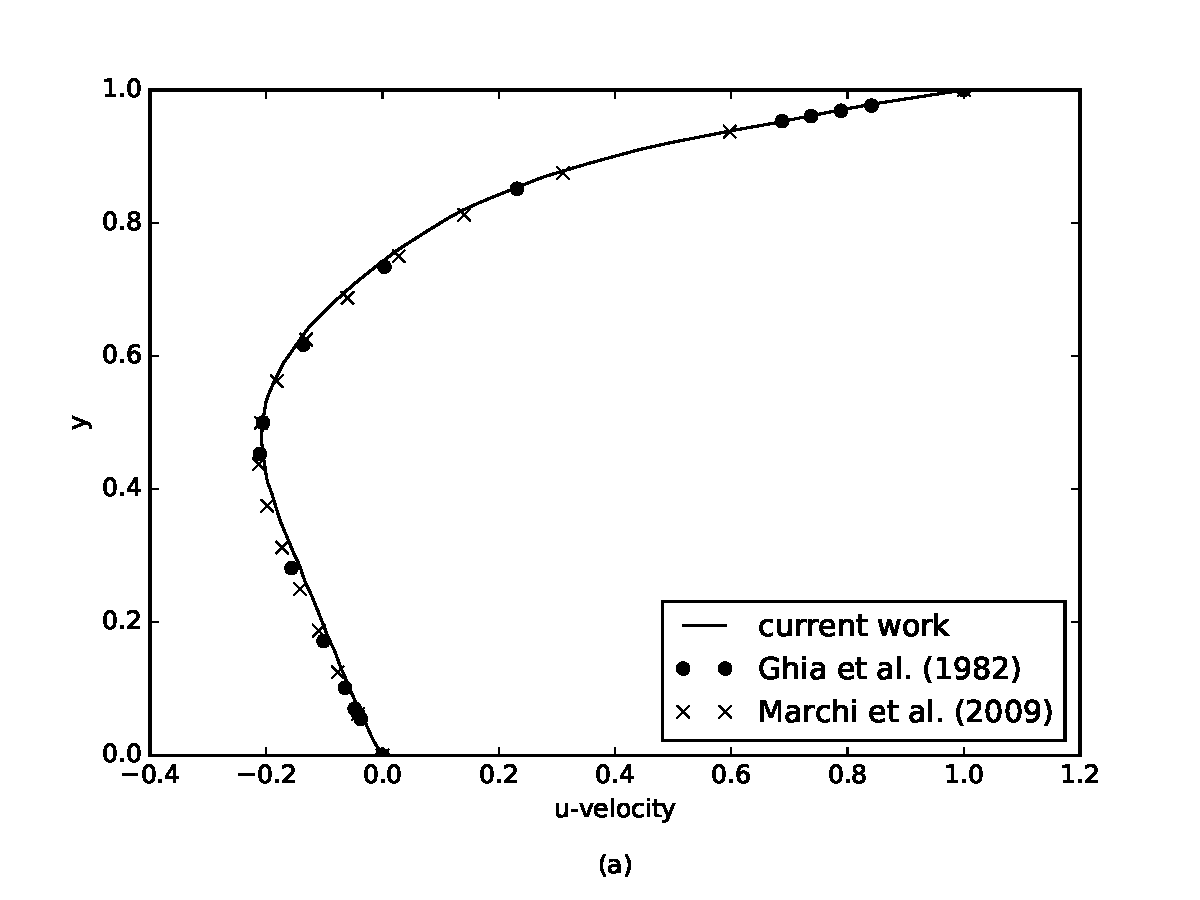
\includegraphics[scale=0.6]{images/Re_100_u_profile.pdf}
\end{figure}
\vspace{-0.2cm}
\centering \scriptsize Centerline $u$ velocity profile ($x=0.5$) in a lid-driven cavity for $Re=100$.
\end{frame}
\fi

%%%%%%%%%%%%%%%%%%%%%%%%%%%%%%%%%%%%%%%%%%%%%%%%%%%%%%%%%%%%%%%%%%%%%%%%%%%%%%%%%%%%%%%%%%
\iffalse
\begin{frame}
 \frametitle{\small Validation - Lid Driven Cavity Flow}
\begin{figure}
  \centering
  \vspace{-1.5cm}
  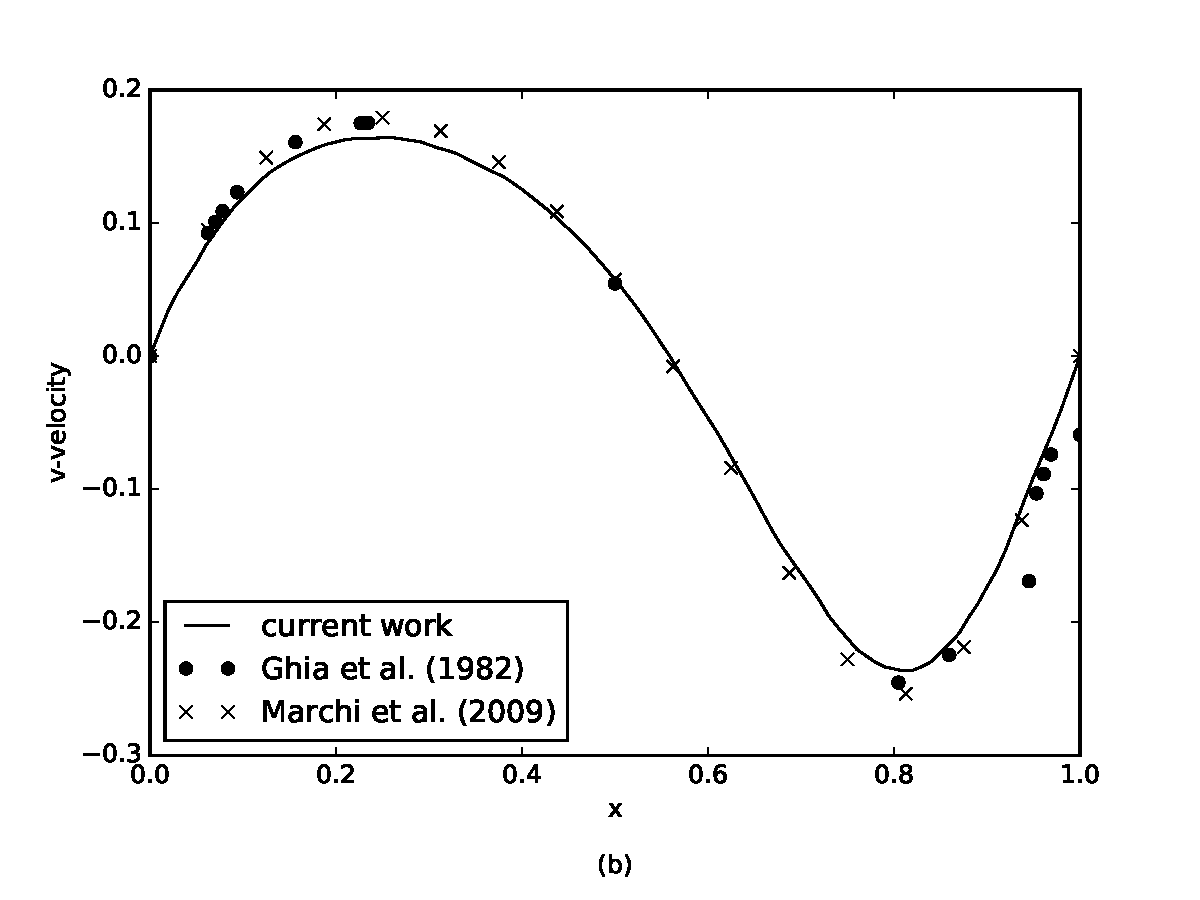
\includegraphics[scale=0.6]{images/Re_100_v_profile.pdf}
\end{figure}
\vspace{-0.2cm}
\centering \scriptsize Centerline $v$ velocity profile ($y=0.5$) in a lid-driven cavity for $Re=100$.
\end{frame}
\fi

%%%%%%%%%%%%%%%%%%%%%%%%%%%%%%%%%%%%%%%%%%%%%%%%%%%%%%%%%%%%%%%%%%%%%%%%%%%%%%%%%%%%%%%%%%

\begin{frame}
 \frametitle{\LARGE Validation - Backward-facing Step}
\begin{center}
 \Huge Coming Soon
\end{center}
\end{frame}


%%%%%%%%%%%%%%%%%%%%%%%%%%%%%%%%%%%%%%%%%%%%%%%%%%%%%%%%%%%%%%%%%%%%%%%%%%%%%%%%%%%%%%%%%%

\begin{frame}
 \frametitle{\LARGE Validation - Pulsation Flow}
\begin{center}
 \Huge Coming Soon
\end{center}
\end{frame}



%%%%%%%%%%%%%%%%%%%%%%%%%%%%%%%%%%%%%%%%%%%%%%%%%%%%%%%%%%%%%%%%%%%%%%%%%%%%%%%%%%%%%%%%%%

\begin{frame}
  \vspace{-1cm}
  \textcolor{gray}{1. Introduction}\\[0.1cm]
  \textcolor{gray}{2. Mathematical Model}\\[0.1cm]
  \textcolor{gray}{3. Validation}\\[0.1cm]
  4. Results\\[0.1cm]
  \textcolor{gray}{5. Conclusion}
\end{frame}

%%%%%%%%%%%%%%%%%%%%%%%%%%%%%%%%%%%%%%%%%%%%%%%%%%%%%%%%%%%%%%%%%%%%%%%%%%%%%%%%%%%%%%%%%%


\begin{frame}
 \frametitle{\LARGE Results}
\begin{center}
 \Huge Coming Soon
\end{center}
\end{frame}


%%%%%%%%%%%%%%%%%%%%%%%%%%%%%%%%%%%%%%%%%%%%%%%%%%%%%%%%%%%%%%%%%%%%%%%%%%%%%%%%%%%%%%%%%%

\iffalse
\begin{frame}
 \frametitle{\LARGE Results}
\begin{figure}
  \vspace{-1cm}
     \centering
     \begin{minipage}{.45\linewidth}
      \centering
      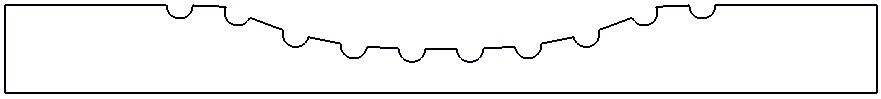
\includegraphics[scale=0.15]{images/CurvedStrut.png}\\
      \scriptsize (a)
     \end{minipage}%
     \begin{minipage}{.45\linewidth}
      \centering
      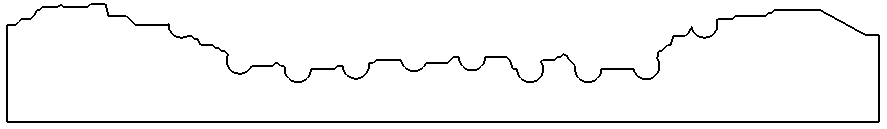
\includegraphics[scale=0.15]{images/RealStrut.png}\\
      \scriptsize (b)
     \end{minipage}
\end{figure}
\vspace{-0.3cm}
\begin{center}
\scriptsize 
     Non-dimensional symmetric geometry for blood flow in coronary artery with drug-eluting stent placed by Wang et al. (2017):
     (a) Curved Channel with Stent
     (b) Real Channel with Stent.
\end{center}
\vspace{0.05cm}
\small
\begin{center}
\begin{columns}[c]
\begin{column}{0.8\textwidth} 
Boundaries Conditions:\\[0.2cm]
Inflow condition: $u=1$, $v=0$ e $\psi=y$;\\[0.1cm]
Outflow condition: $\psi=y$;\\[0.1cm]
Top plate: $u=0$, $v=0$, $\psi=1$;\\[0.1cm]
Symmetry condition: $v=0$, $\psi=0$; \\[0.1cm]
Drug-eluting stent: $u=0$, $v=0$, $\psi=1$ e $c=1$
\end{column}
\hspace{-1cm}
\begin{column}{0.3\textwidth}
$R=0.0015m$\\[0.1cm]
$\mu=0.0035Pa.s$\\[0.1cm]
$\rho=1060kg/m^3$\\[0.1cm]\\
$u=12cm/s$\\[0.1cm]
$Re=54.5$
\end{column}
\end{columns}
\end{center}
\end{frame}
\fi


%%%%%%%%%%%%%%%%%%%%%%%%%%%%%%%%%%%%%%%%%%%%%%%%%%%%%%%%%%%%%%%%%%%%%%%%%%%%%%%%%%%%%%%%%%

\iffalse
\begin{frame}
 \frametitle{\LARGE Results}
\begin{figure}
     \begin{minipage}{.50\linewidth}
      \centering
      
\includegraphics[scale=0.08]{images/vel_RealStrut200.png}\\
      \scriptsize t = 0.1
     \end{minipage}%
     \begin{minipage}{.50\linewidth}
      \centering
      
\includegraphics[scale=0.08]{images/vel_RealStrut1000.png}\\
      \scriptsize t = 0.5
     \end{minipage}
     \begin{minipage}{.50\linewidth}
     \medskip
      \centering
      
\includegraphics[scale=0.08]{images/vel_RealStrut2000.png}\\
      \scriptsize t = 1.0
     \end{minipage}%
     \begin{minipage}{.50\linewidth}
     \medskip
      \centering
      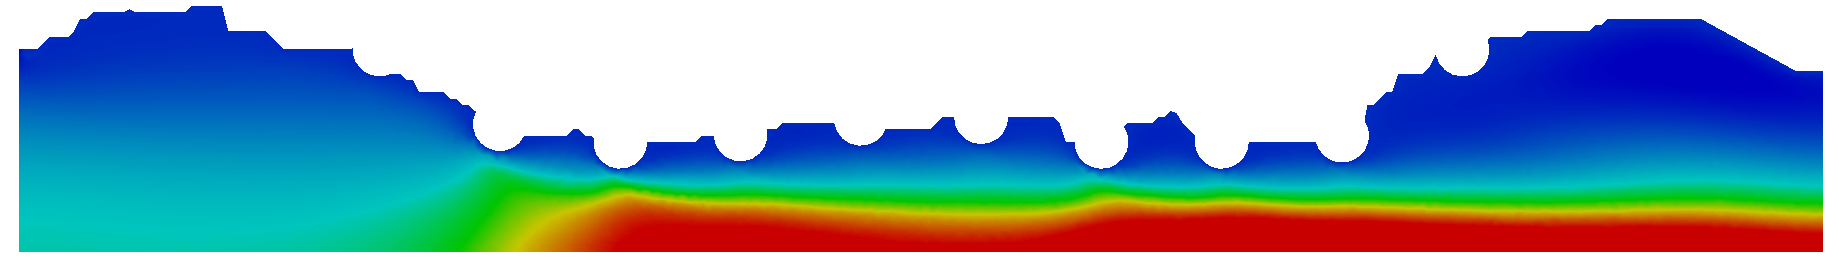
\includegraphics[scale=0.08]{images/vel_RealStrut6000.png}\\
      \scriptsize t = 3.0
     \end{minipage}
     \begin{minipage}{.50\linewidth}
      \centering
      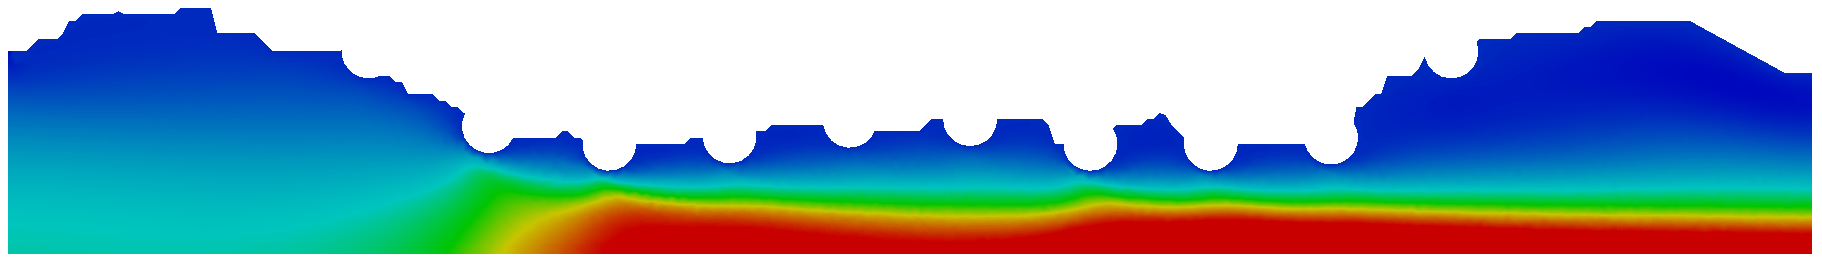
\includegraphics[scale=0.08]{images/vel_RealStrut8000.png}\\
      \scriptsize t = 4.0
     \end{minipage}%
     \begin{minipage}{.50\linewidth}
      \centering
      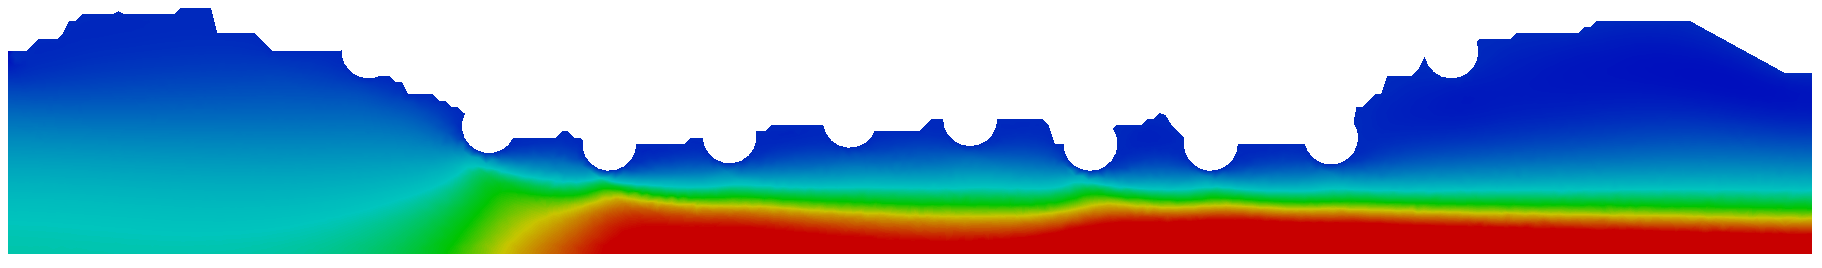
\includegraphics[scale=0.08]{images/vel_RealStrut10000.png}\\
      \scriptsize t = 5.0
 \end{minipage}
     \begin{minipage}{.50\linewidth}
     \medskip
      \centering
      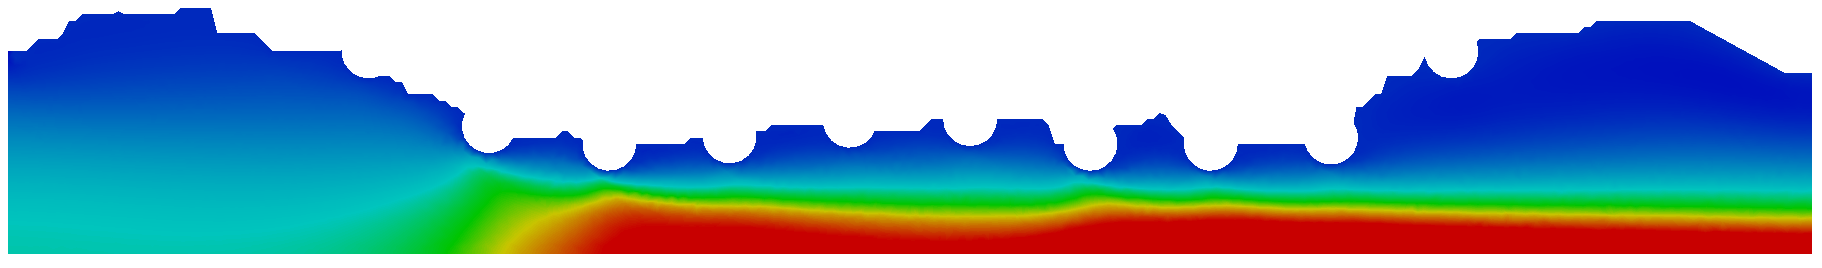
\includegraphics[scale=0.08]{images/vel_RealStrut14000.png}\\
      \scriptsize t = 7.0
     \end{minipage}%
     \begin{minipage}{.50\linewidth}
     \medskip
      \centering
      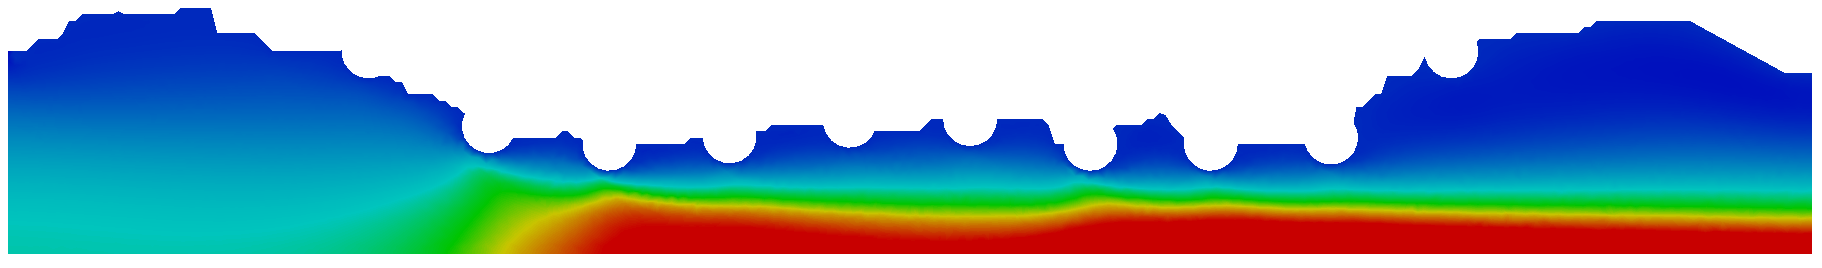
\includegraphics[scale=0.08]{images/vel_RealStrut20000.png}\\
      \scriptsize t = 10.0
     \end{minipage}
\end{figure}
\vspace{0cm}
\centering \scriptsize Evolution in time and space of velocity field
\end{frame}
\fi

%%%%%%%%%%%%%%%%%%%%%%%%%%%%%%%%%%%%%%%%%%%%%%%%%%%%%%%%%%%%%%%%%%%%%%%%%%%%%%%%%%%%%%%%%%

\iffalse
\begin{frame}
 \frametitle{\LARGE Results - Velocity Field}

\vspace{-0.8cm}
\begin{figure}
     \begin{minipage}{.50\linewidth}
      \centering
      
\includegraphics[scale=0.075]{images/vel_CurvedStrut2000.png}\\
      \tiny t = 1.0
     \end{minipage}%
     \begin{minipage}{.50\linewidth}
      \centering
      
\includegraphics[scale=0.075]{images/vel_RealStrut2000.png}\\
      \tiny t = 1.0
     \end{minipage}
     \begin{minipage}{.50\linewidth}
     \smallskip
      \centering
      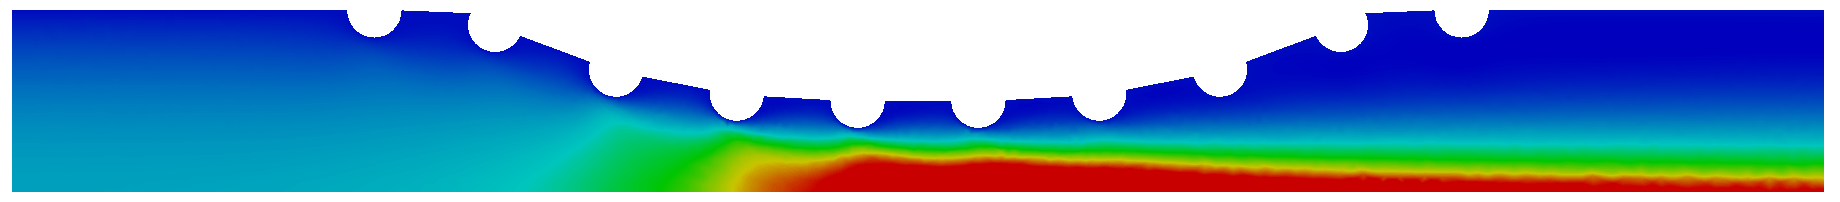
\includegraphics[scale=0.075]{images/vel_CurvedStrut10000.png}\\
      \tiny t = 5.0
     \end{minipage}%
     \begin{minipage}{.50\linewidth}
     \smallskip
      \centering
      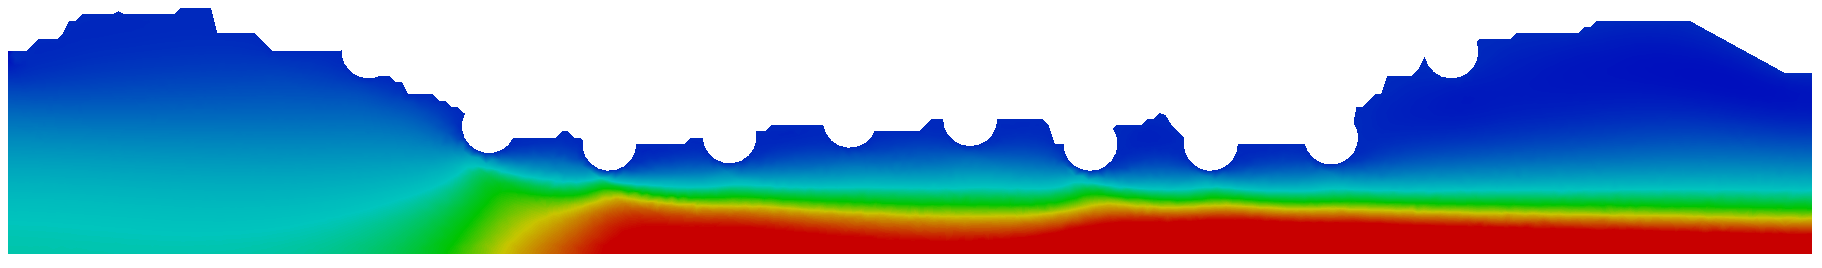
\includegraphics[scale=0.075]{images/vel_RealStrut10000.png}\\
      \tiny t = 5.0
     \end{minipage}
     \begin{minipage}{.50\linewidth}
      \centering
      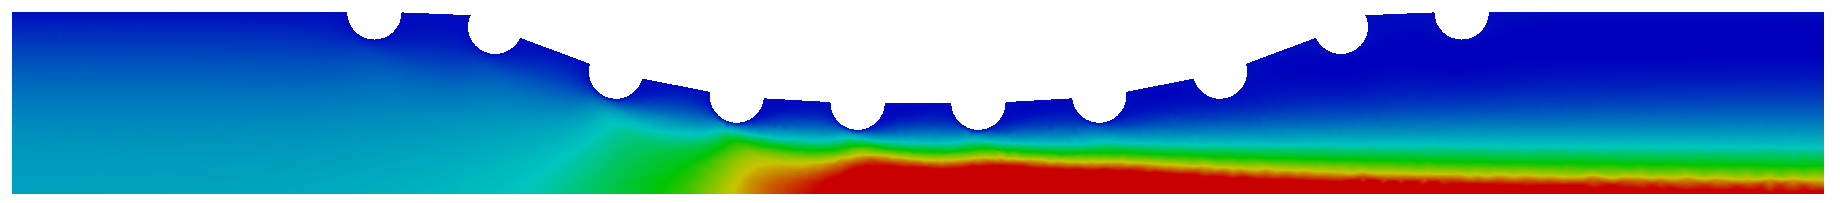
\includegraphics[scale=0.075]{images/vel_CurvedStrut20000.png}\\
      \tiny t = 10.0
     \end{minipage}%
     \begin{minipage}{.50\linewidth}
      \centering
      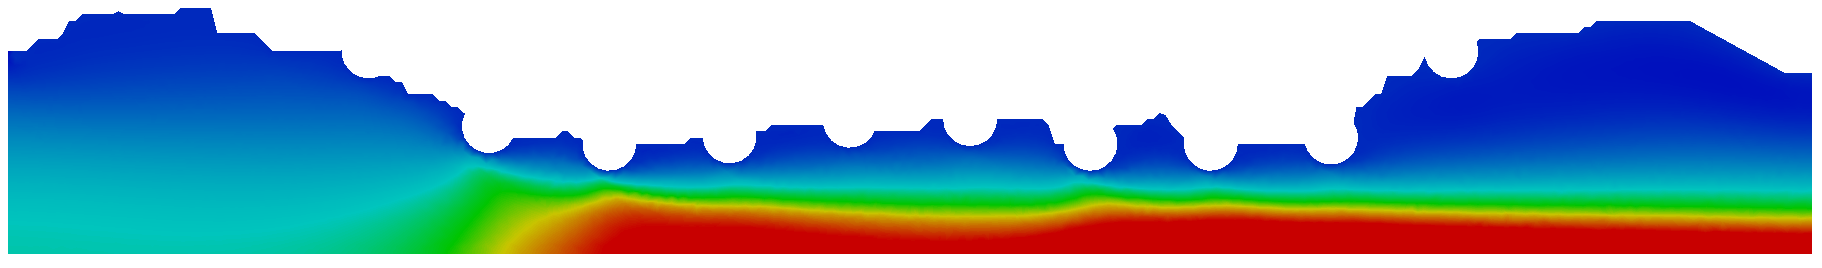
\includegraphics[scale=0.075]{images/vel_RealStrut20000.png}\\
      \tiny t = 10.0
     \end{minipage}
\end{figure}
\vspace{-0.2cm}
\centering \tiny Evolution in time and space of velocity field:\\
                 Curved Channel (left column) and Real Channel (right column)
\vspace{-0.5cm}
\begin{figure}
     \begin{minipage}{.50\linewidth}
     \medskip
      \centering
      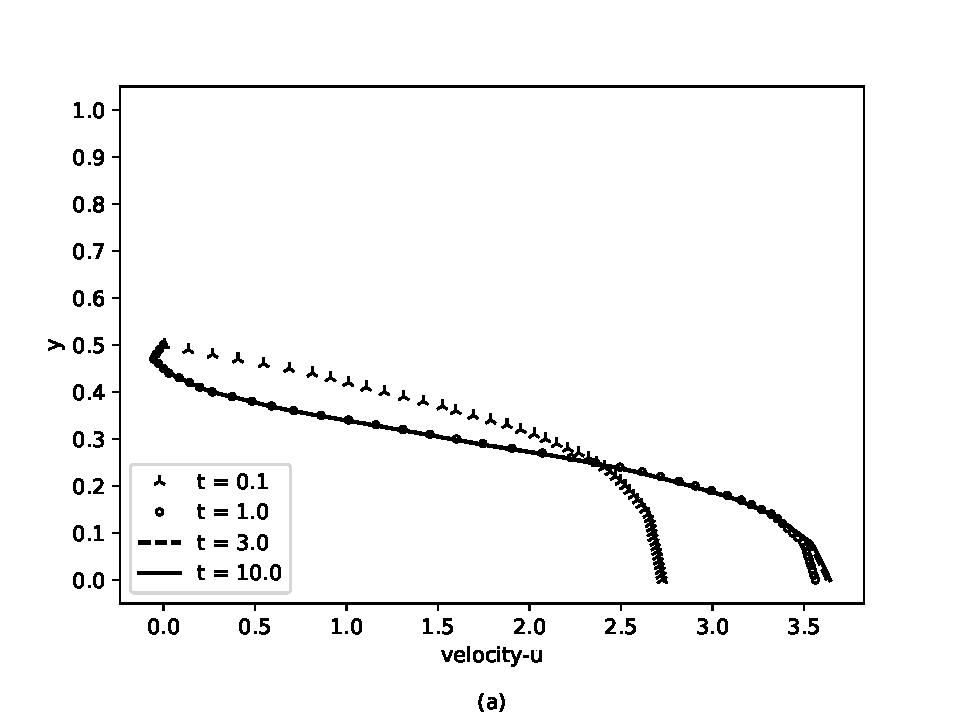
\includegraphics[scale=0.35]{images/vel_CurvedStrut_evol.pdf}\\
     \end{minipage}%
     \begin{minipage}{.50\linewidth}
     \medskip
      \centering
      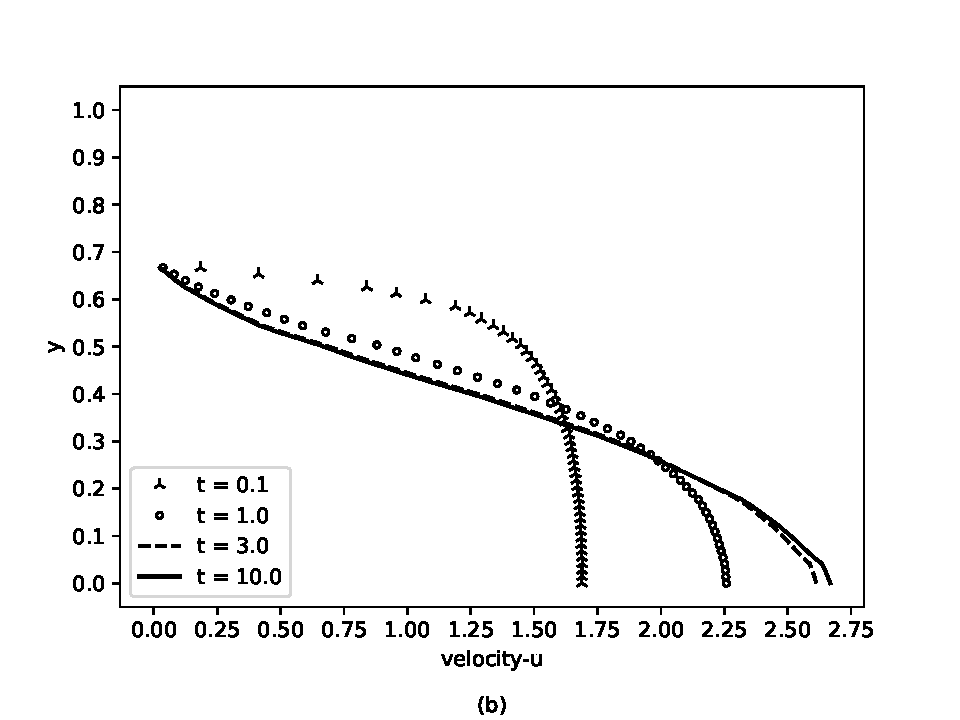
\includegraphics[scale=0.35]{images/vel_RealStrut_evol.pdf}\\
     \end{minipage}
\end{figure}
\vspace{-0.2cm}
\centering \tiny Evolution of velocity profile in centerline ($x=0.5L$):\\
                       (a) Curved Channel and (b) Real Channel
\end{frame}
\fi

%%%%%%%%%%%%%%%%%%%%%%%%%%%%%%%%%%%%%%%%%%%%%%%%%%%%%%%%%%%%%%%%%%%%%%%%%%%%%%%%%%%%%%%%%%

\iffalse
\begin{frame}
 \frametitle{\LARGE Results - Concentration Field}
\vspace{-0.7cm}
\begin{figure}
     \begin{minipage}{.50\linewidth}
      \centering
      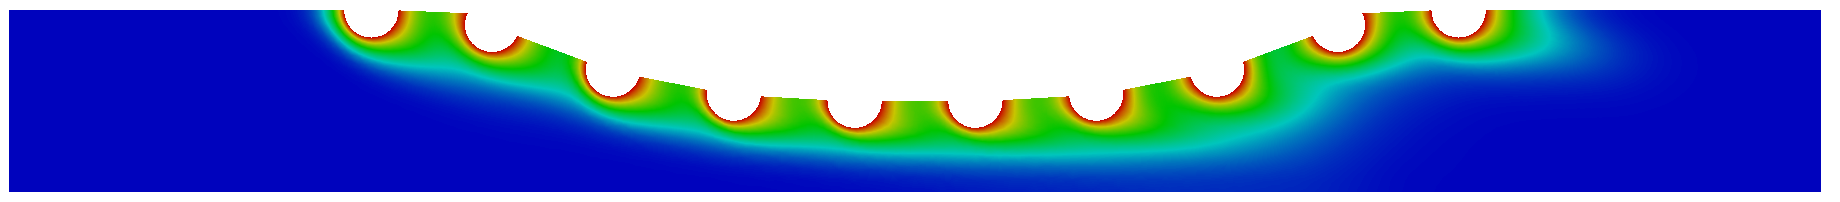
\includegraphics[scale=0.075]{images/conc1_CurvedStrut2000.png}\\
      \tiny t = 1.0
     \end{minipage}%
     \begin{minipage}{.50\linewidth}
      \centering
      
\includegraphics[scale=0.075]{images/conc10_CurvedStrut5000.png}\\
      \tiny t = 1.0
     \end{minipage}
     \begin{minipage}{.50\linewidth}
     \medskip
      \centering
      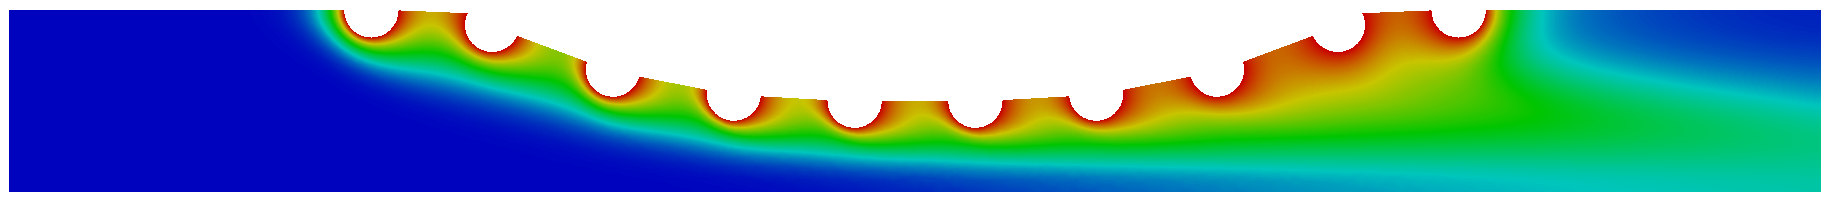
\includegraphics[scale=0.075]{images/conc1_CurvedStrut10000.png}\\
      \tiny t = 5.0
     \end{minipage}%
     \begin{minipage}{.50\linewidth}
     \medskip
      \centering
      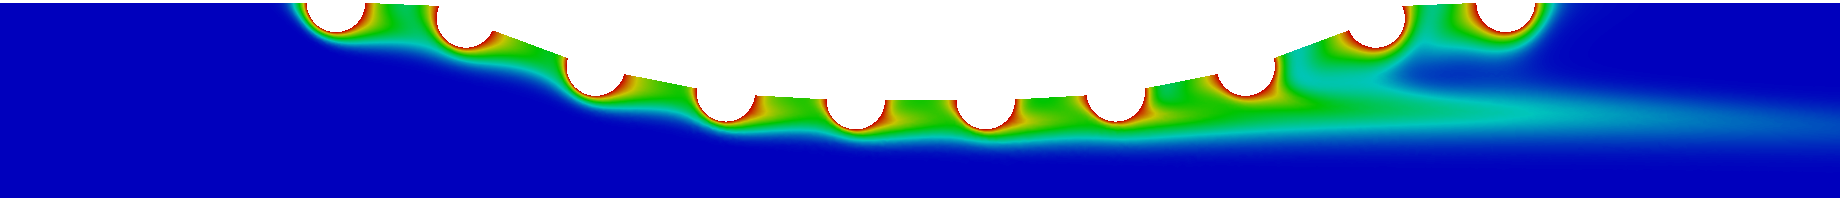
\includegraphics[scale=0.075]{images/conc10_CurvedStrut25000.png}\\
      \tiny t = 5.0
     \end{minipage}
     \begin{minipage}{.50\linewidth}
      \centering
      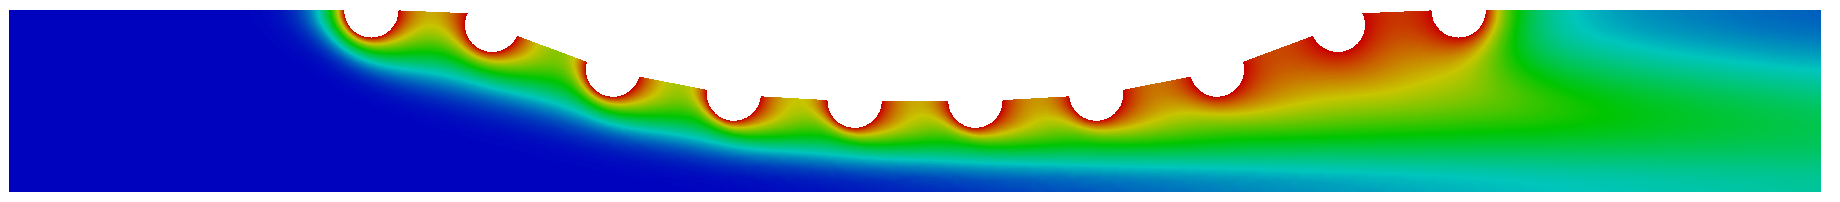
\includegraphics[scale=0.075]{images/conc1_CurvedStrut20000.png}\\
      \tiny t = 10.0
     \end{minipage}%
     \begin{minipage}{.50\linewidth}
      \centering
      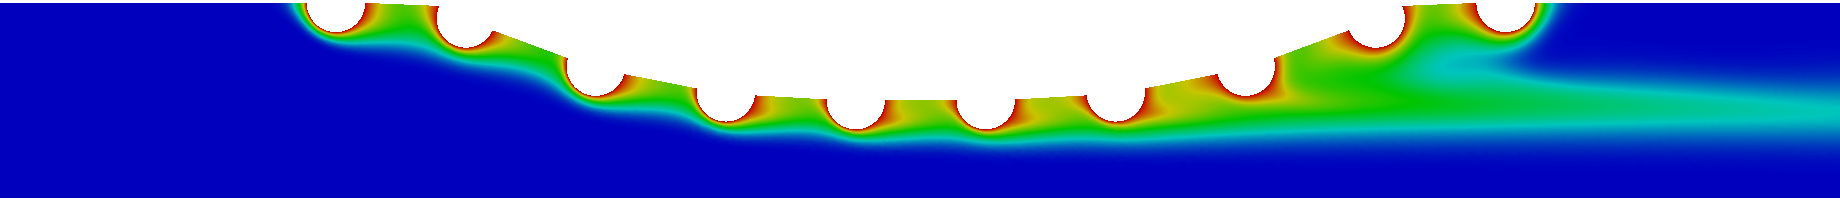
\includegraphics[scale=0.075]{images/conc10_CurvedStrut50000.png}\\
      \tiny t = 10.0
     \end{minipage}
\end{figure}
\vspace{-0.2cm}
\centering \scriptsize Evolution in time and space of concentration field in Curved Channel:\\
                 $Sc=1$ (left column) and $Sc=10$ (right column)
\vspace{0cm}
\begin{figure}
     \begin{minipage}{.50\linewidth}
      \centering
      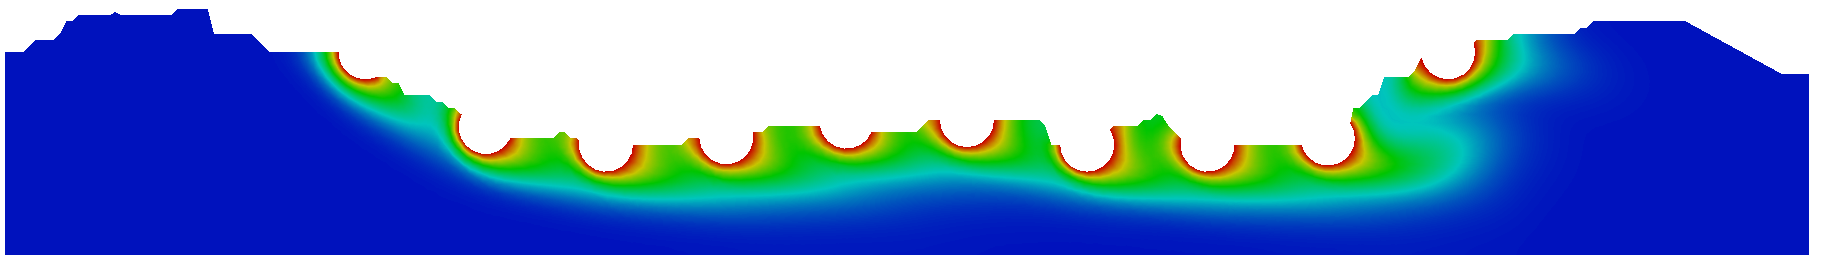
\includegraphics[scale=0.075]{images/conc1_RealStrut2000.png}\\
      \tiny t = 1.0
     \end{minipage}%
     \begin{minipage}{.50\linewidth}
      \centering
      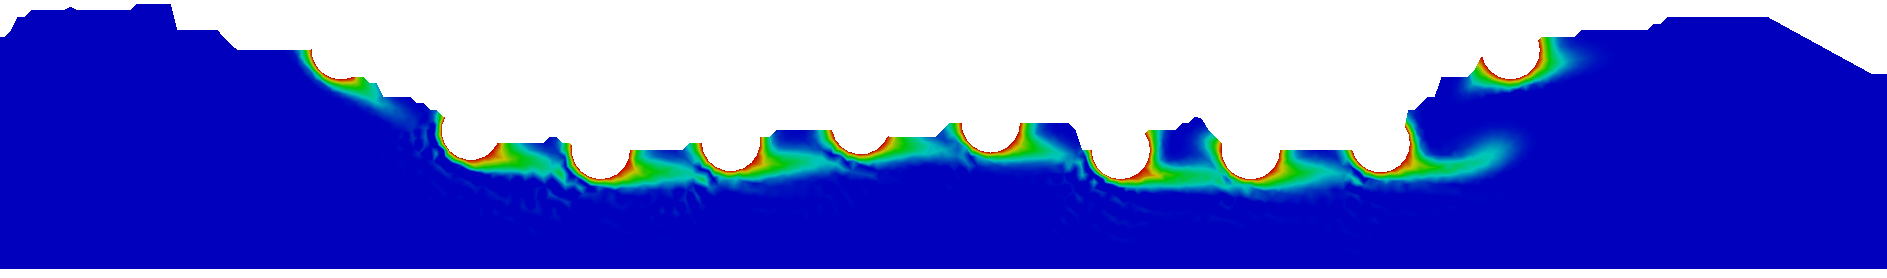
\includegraphics[scale=0.075]{images/conc10_RealStrut5000.png}\\
      \tiny t = 1.0
     \end{minipage}
     \begin{minipage}{.50\linewidth}
     \medskip
      \centering
      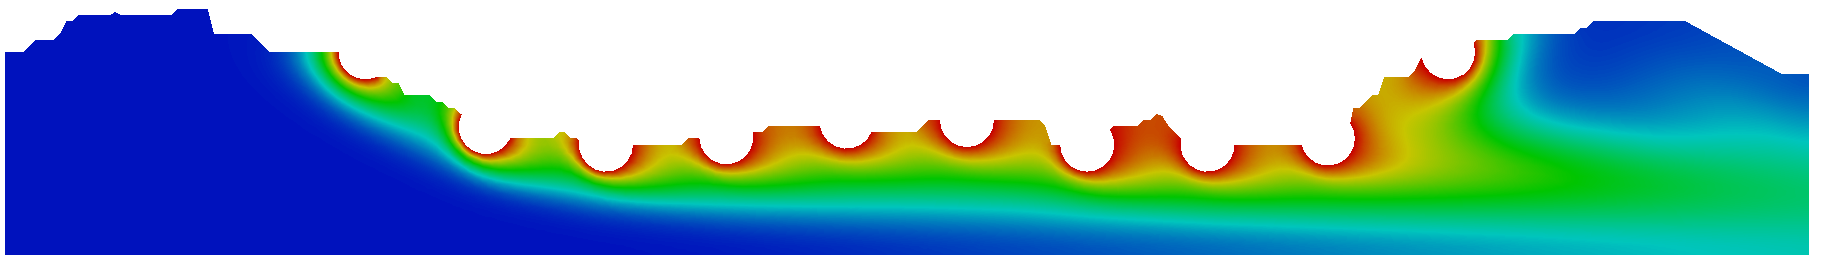
\includegraphics[scale=0.075]{images/conc1_RealStrut10000.png}\\
      \tiny t = 5.0
     \end{minipage}%
     \begin{minipage}{.50\linewidth}
     \medskip
      \centering
      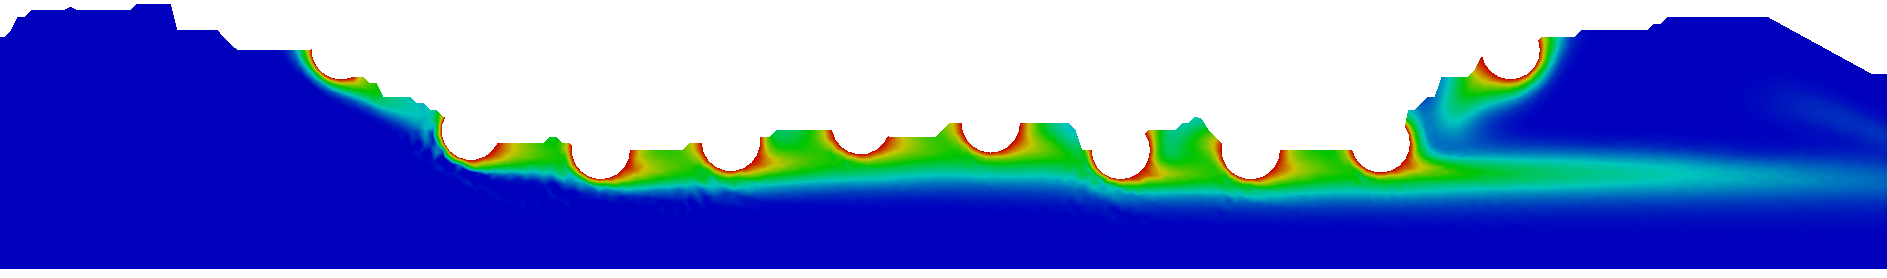
\includegraphics[scale=0.075]{images/conc10_RealStrut25000.png}\\
      \tiny t = 5.0
     \end{minipage}
     \begin{minipage}{.50\linewidth}
      \centering
      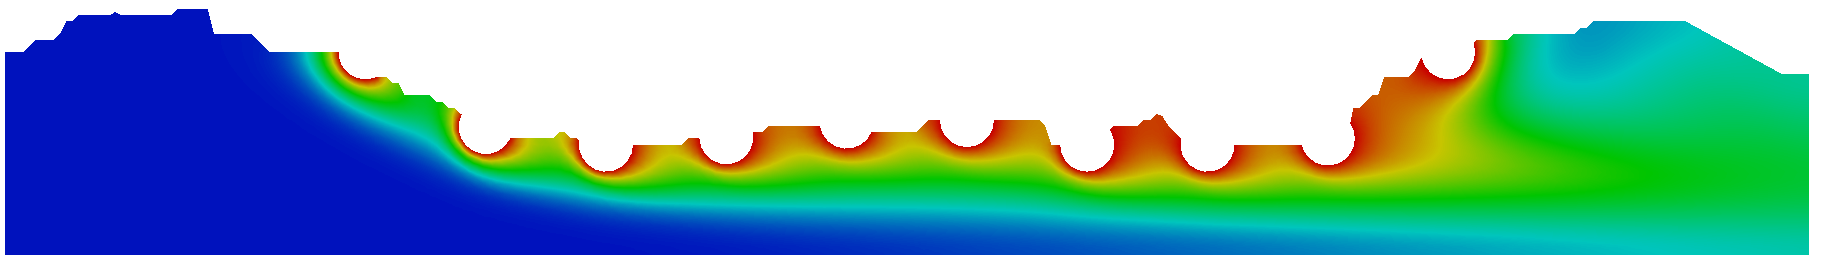
\includegraphics[scale=0.075]{images/conc1_RealStrut20000.png}\\
      \tiny t = 10.0
     \end{minipage}%
     \begin{minipage}{.50\linewidth}
      \centering
      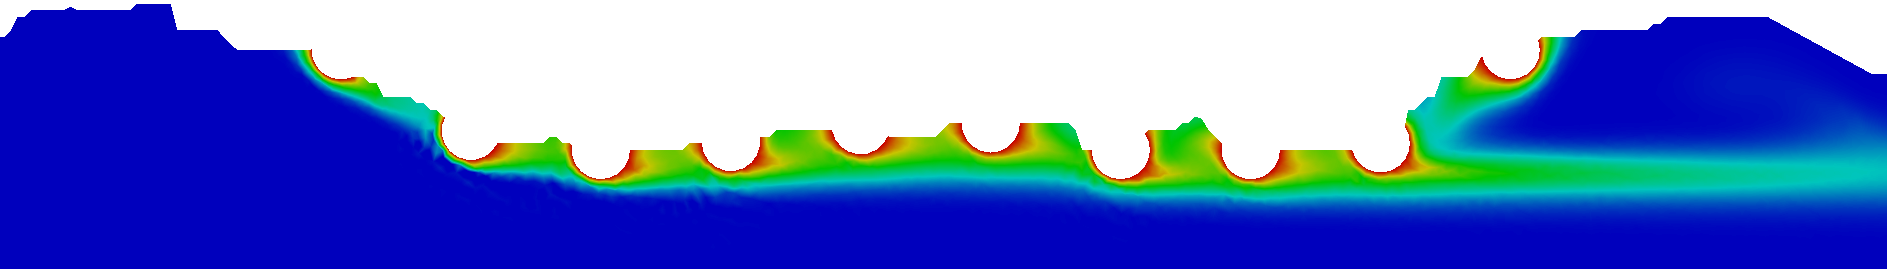
\includegraphics[scale=0.075]{images/conc10_RealStrut50000.png}\\
      \tiny t = 10.0
     \end{minipage}
\end{figure}
\vspace{-0.2cm}
\centering \scriptsize Evolution in time and space of concentration field in Real Channel:\\
                 $Sc=1$ (left column) and $Sc=10$ (right column)
\end{frame}
\fi

%%%%%%%%%%%%%%%%%%%%%%%%%%%%%%%%%%%%%%%%%%%%%%%%%%%%%%%%%%%%%%%%%%%%%%%%%%%%%%%%%%%%%%%%%%

\begin{frame}
  \vspace{-1cm}
  \textcolor{gray}{1. Introduction}\\[0.1cm]
  \textcolor{gray}{2. Mathematical Model}\\[0.1cm]
  \textcolor{gray}{3. Validation}\\[0.1cm]
  \textcolor{gray}{4. Results}\\[0.1cm]
  5. Conclusion
\end{frame}

%%%%%%%%%%%%%%%%%%%%%%%%%%%%%%%%%%%%%%%%%%%%%%%%%%%%%%%%%%%%%%%%%%%%%%%%%%%%%%%%%%%%%%%%%%

\begin{frame}
 \frametitle{\LARGE Conclusion}
 \vspace{-1cm}
\begin{enumerate}
 \justifying
 \small
% \item Was observed that the species transport in blood flow is directly influenced
%       by drug used in stent production\\

% \vspace{0.3cm}
 
 \item The streamfunction-vorticity formulation showed an useful approach for to calculate
       the velocity and concentration fields since the variables are scalars allowing a
       smooth implementation\\

 \vspace{0.3cm}

 \item Due to generalized construction of the code, the simulator is able to describe
       drug-eluting stent problem in coronary artery as well as flows of Newtonian fluids
       with scalar transport (concentration or temperature)\\

 \vspace{0.3cm}

 \item The ALE description allows moving boundary problems to be simulated
\end{enumerate}
\end{frame}


%%%%%%%%%%%%%%%%%%%%%%%%%%%%%%%%%%%%%%%%%%%%%%%%%%%%%%%%%%%%%%%%%%%%%%%%%%%%%%%%%%%%%%%%%%

\begin{frame}
 \centering
 \vspace{-1cm}
 \Huge Thank you!\\
 \vspace{0.5cm}
 \small marquesleandro67@gmail.com\\
 \small gustavo.rabello@mecanica.coppe.ufrj.br\\
 \small jose.pontes@uerj.br\\
 \vspace{1.0cm}
 \small The authors thank the FAPERJ (Research Support Foundation of the State of Rio de Janeiro)
        for its financial support

 \vspace{-0.2cm}
 \begin{figure}
  \centering
  
\includegraphics[scale=0.4]{images/faperj.jpg}\\
 \end{figure}
\end{frame}




\end{document}
%%%%%%%%%%%%%%%%%%%%%%%%%%%%%%%%%%%%%%%%%%%%%%%%%%%%%%%%%%%%%%%%%%%%%%%%%%%%%%%%%%%%%%%%%%
